%\documentclass{beamer}
\documentclass[aspectratio=169]{beamer}
 
\usepackage[utf8]{inputenc}
\usetheme{Madrid}

\usepackage{biblatex}

\usepackage{mathrsfs}

\usepackage[symbols,nogroupskip,nonumberlist,sort=use]{glossaries-extra}
\usepackage{amsmath}
\usepackage{amsfonts}
\usepackage{amssymb}
\usepackage{siunitx}
\usepackage{transparent}
\usepackage{longtable,booktabs}

\usepackage{chronology}
\usepackage{epigraph}

\usepackage{subfig}

\usepackage{caption} 
\captionsetup[table]{skip=5pt}

\sisetup{math-micro=\text{µ},text-micro=µ}
\glsxtrnewsymbol[description={Signal Segment Size}]{w}{\ensuremath{w}}
\glsxtrnewsymbol[description={Length in sample points of the Segment}]{N}{\ensuremath{N}}
\glsxtrnewsymbol[description={Number of available channels}]{C}{\ensuremath{C}}
\glsxtrnewsymbol[description={Signal Span}]{lambda}{\ensuremath{\lambda}}
\glsxtrnewsymbol[description={Sampling Frequency}]{Fs}{\ensuremath{F_s}}
\glsxtrnewsymbol[description={Length in pixel of the unit-scale patch}]{Deltas}{\ensuremath{\Delta_s}}
\glsxtrnewsymbol[description={Peak-to-peak Amplitude}]{DeltamuV}{\ensuremath{\Delta \mu V}}
\glsxtrnewsymbol[description={Signal Amplitude Scale Factor}]{gamma}{\ensuremath{\gamma}}
\glsxtrnewsymbol[description={Time Scale Factor}]{gammat}{\ensuremath{\gamma_t}}
\glsxtrnewsymbol[description={Image Height}]{Hy}{\ensuremath{H_y}}
\glsxtrnewsymbol[description={Image Width}]{Wx}{\ensuremath{W_x}}
\glsxtrnewsymbol[description={Horizontal Patch Scale}]{St}{\ensuremath{S_t}}
\glsxtrnewsymbol[description={Vertical Patch Scale}]{Sv}{\ensuremath{S_v}}
\glsxtrnewsymbol[description={Patch Height}]{Sy}{\ensuremath{\mathbf{S}_y}}
\glsxtrnewsymbol[description={Patch Width}]{Sx}{\ensuremath{\mathbf{S}_x}}
\glsxtrnewsymbol[description={Keypoint}]{kp}{\ensuremath{\mathbf{kp}}}
\glsxtrnewsymbol[description={Pixel}]{P}{\ensuremath{\mathbf{p}}}
\glsxtrnewsymbol[description={Descriptor}]{d}{\ensuremath{\mathbf{d}}}
\glsxtrnewsymbol[description={Keypoint Density}]{kpd}{\ensuremath{\mathbf{kp_d}}}
\glsxtrnewsymbol[description={Intensification Sequences Repetitions}]{ka}{\ensuremath{k_a}}
\glsxtrnewsymbol[description={Best Performing Channel}]{bpc}{\ensuremath{bpc}}
\glsxtrnewsymbol[description={Number of k-Neighbors}]{k}{\ensuremath{k}}
\glsxtrnewsymbol[description={Template Dictionary}]{T}{\ensuremath{T}}

\DeclareMathOperator*{\argmin}{arg\,min}


\newcommand*{\TitleFont}{%
      \usefont{\encodingdefault}{\rmdefault}{b}{n}%
      \fontsize{9}{20}%
      \selectfont}
      
    
%\renewcommand{\figurename}{Fig.}  
\usepackage[figurename=]{caption}

\newcommand\Fontvi{\fontsize{13}{13.2}\selectfont}
\newcommand\Fontre{\fontsize{16}{16.2}\selectfont}

\renewcommand{\contentsname}{\centering Contents}

\newsavebox{\authbox}
\sbox{\authbox}{%
\centering
\begin{minipage}{0.33\linewidth}
\centering\normalsize
Supervisor \par
Dr. Juan Miguel Santos
\end{minipage}
\begin{minipage}{0.33\linewidth}
\centering\normalsize
Candidate \par
\underline{Ing. Rodrigo Ramele}
\end{minipage}
\hfill
\begin{minipage}{0.33\linewidth}
\centering\normalsize
Cosupervisor \par
Dra. Ana Julia Villar
\end{minipage}
}
 
%Information to be included in the title page:
\title[HIST of EEG for BCI] %optional
{Histogram of Gradient Orientations of EEG Signal Plots for Brain Computer Interfaces}
 
\subtitle{Dissertation Defense}
 
\author[Ramele, Rodrigo]{ % (optional, for multiple authors)
\usebox{\authbox}
}
 
\institute[ITBA] % (optional)
{
\begin{columns}
\begin{column}{0.4\textwidth}
\hfill 
\includegraphics[scale=.20]{images/itbalogo.png}
\end{column}
\begin{column}{0.6\textwidth}
\Fontvi
Doctorado en Ingeniería en Informática\\
Instituto Tecnológico de Buenos Aires
\end{column}
\end{columns}
}
 
\date[Nov 29, 2018] % (optional)
{Noviembre 29 2018}


 
%\logo{
\includegraphics[height=1.0cm]{images/itbalogo.png}}
 
\bibliography{Bibliography}


 
\begin{document}

%{
%\usebackgroundtemplate{\transparent{0.1}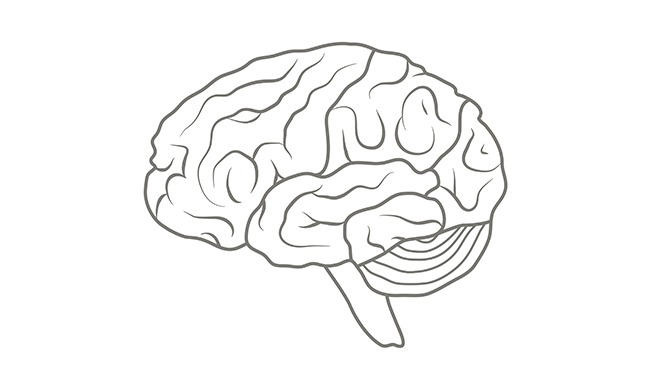
\includegraphics[width=\paperwidth]{images/brainback.png}} 
%\frame{\titlepage}
%}

\begin{frame}
\titlepage
\begin{center}
%
\includegraphics[scale=0.05]{images/itba.pdf}	
%
\includegraphics[height=2.0cm]{images/itbalogo.png}	
\end{center}
\end{frame}


\begin{frame}
\begin{center}
\frametitle{Outline}
\tableofcontents{}
\end{center}
\end{frame}
    
    
%\section{Introduction}
%\begin{frame}
%\frametitle{Brain Computer Interfaces}
%\begin{center}
%\begin{figure}[]
%\centering
%\only<1>{\subfloat[Fig. 1]{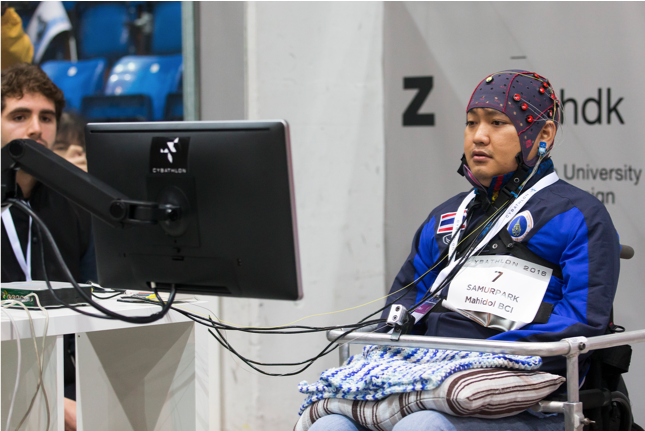
\includegraphics[height=3.8cm,width=7cm]{images/Cybathlon.png}}}
%\only<1>{\subfloat[Fig. 1]{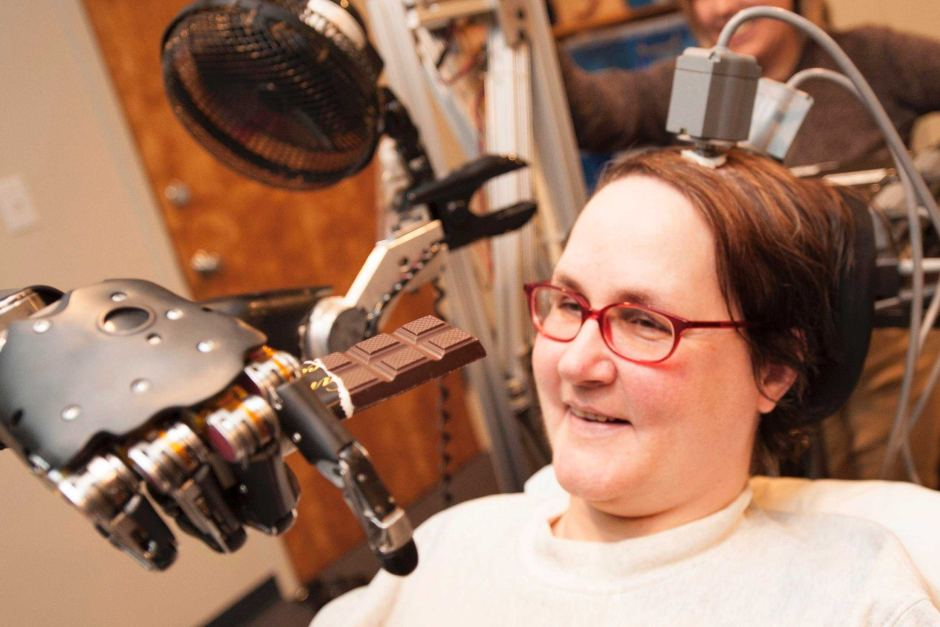
\includegraphics[height=3.8cm,width=7cm]{images/Jane.jpg}}}\\
%\only<1>{\subfloat[Fig. 1]{\includegraphics[height=3.8cm,width=7cm]{images/gTecEEGSubject.png}}}
%\only<1>{\subfloat[Fig. 1]{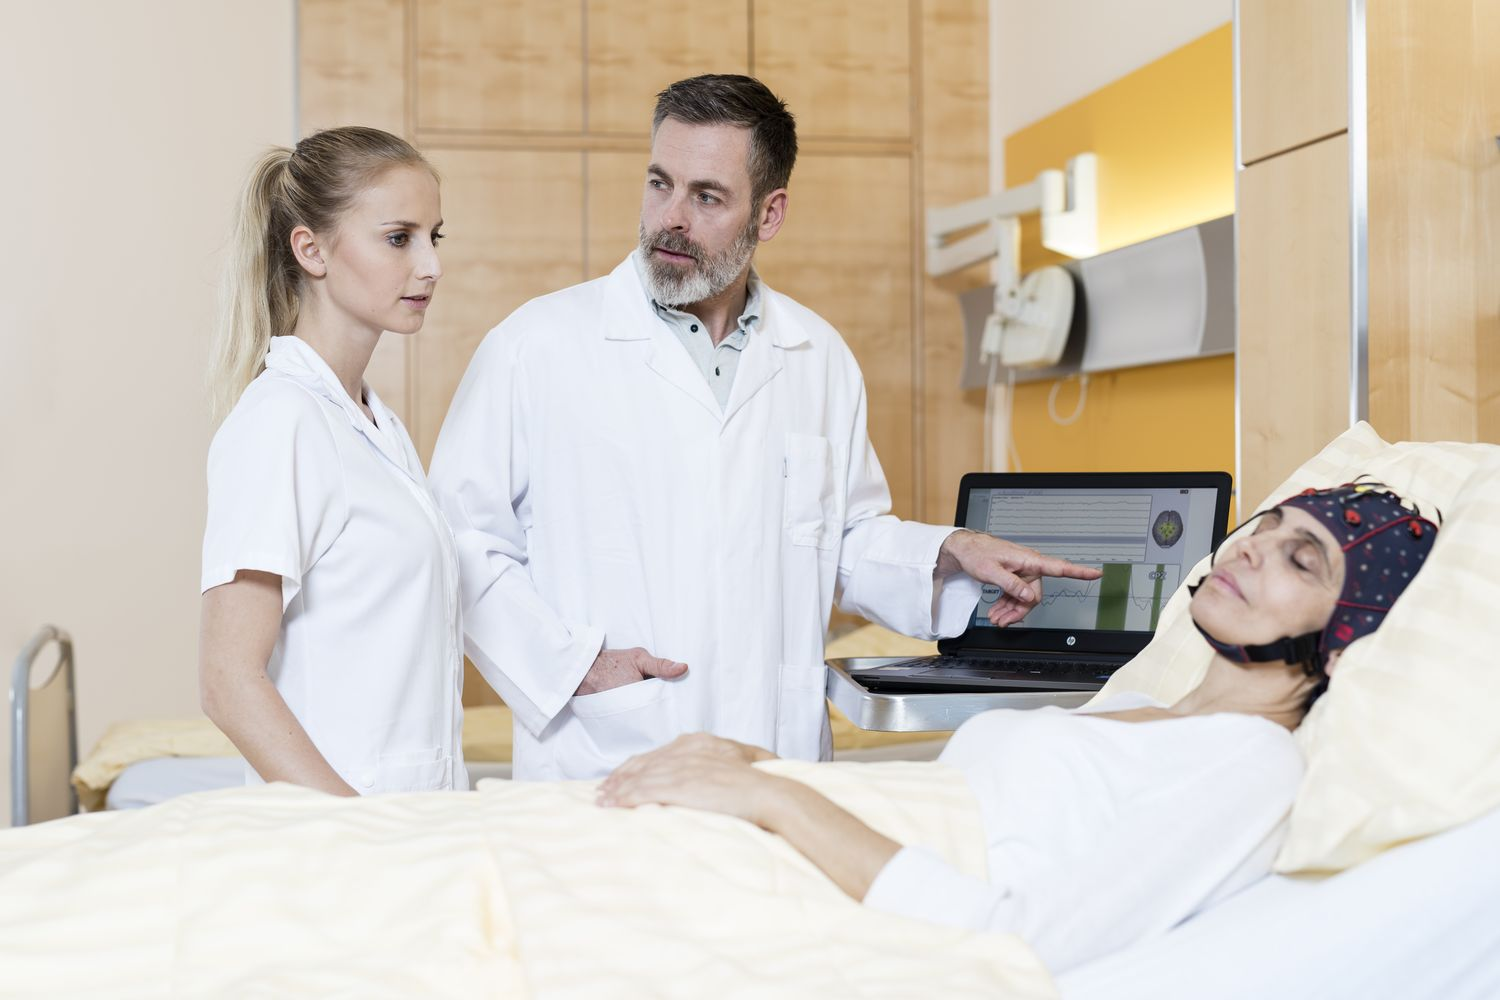
\includegraphics[height=3.8cm,width=7cm]{images/DoC.jpg}}}
%\caption[Wearable portable Digital Electroencephalograph]{Digital and wearable electroencephalographs.}
%\label{fig:digitalelectroencephalograph}
%\end{figure}
%\end{center}
%\end{frame}


\section{Introduction}
\begin{frame}
\frametitle{Brain Computer Interfaces - Current trends}
\begin{center}
\begin{figure}[]
\centering
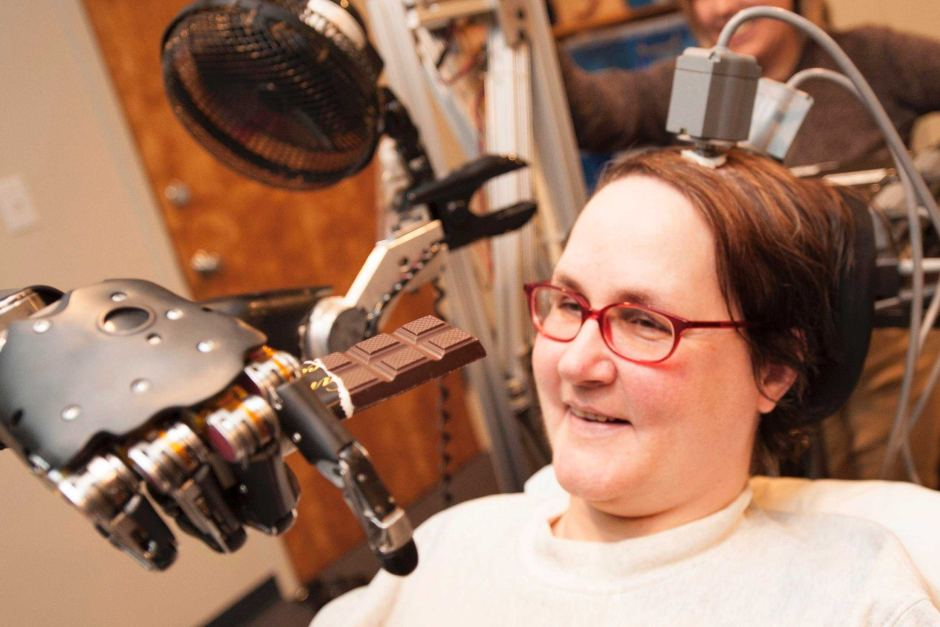
\includegraphics[height=3.5cm,width=7cm]{images/Jane.jpg}
\includegraphics[height=3.5cm,width=7cm]{images/gTecEEGSubject.png}\\
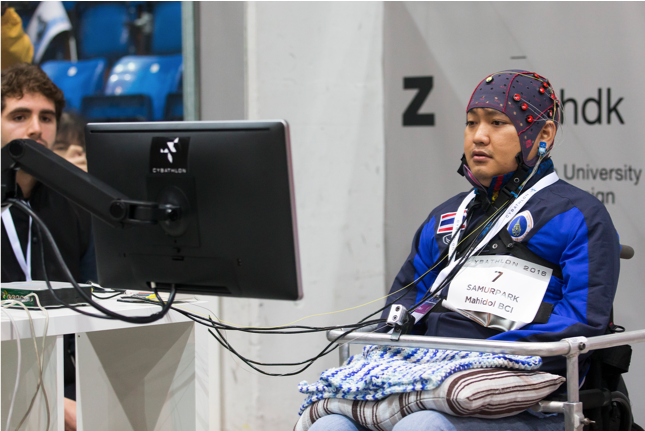
\includegraphics[height=3.5cm,width=7cm]{images/Cybathlon.png}
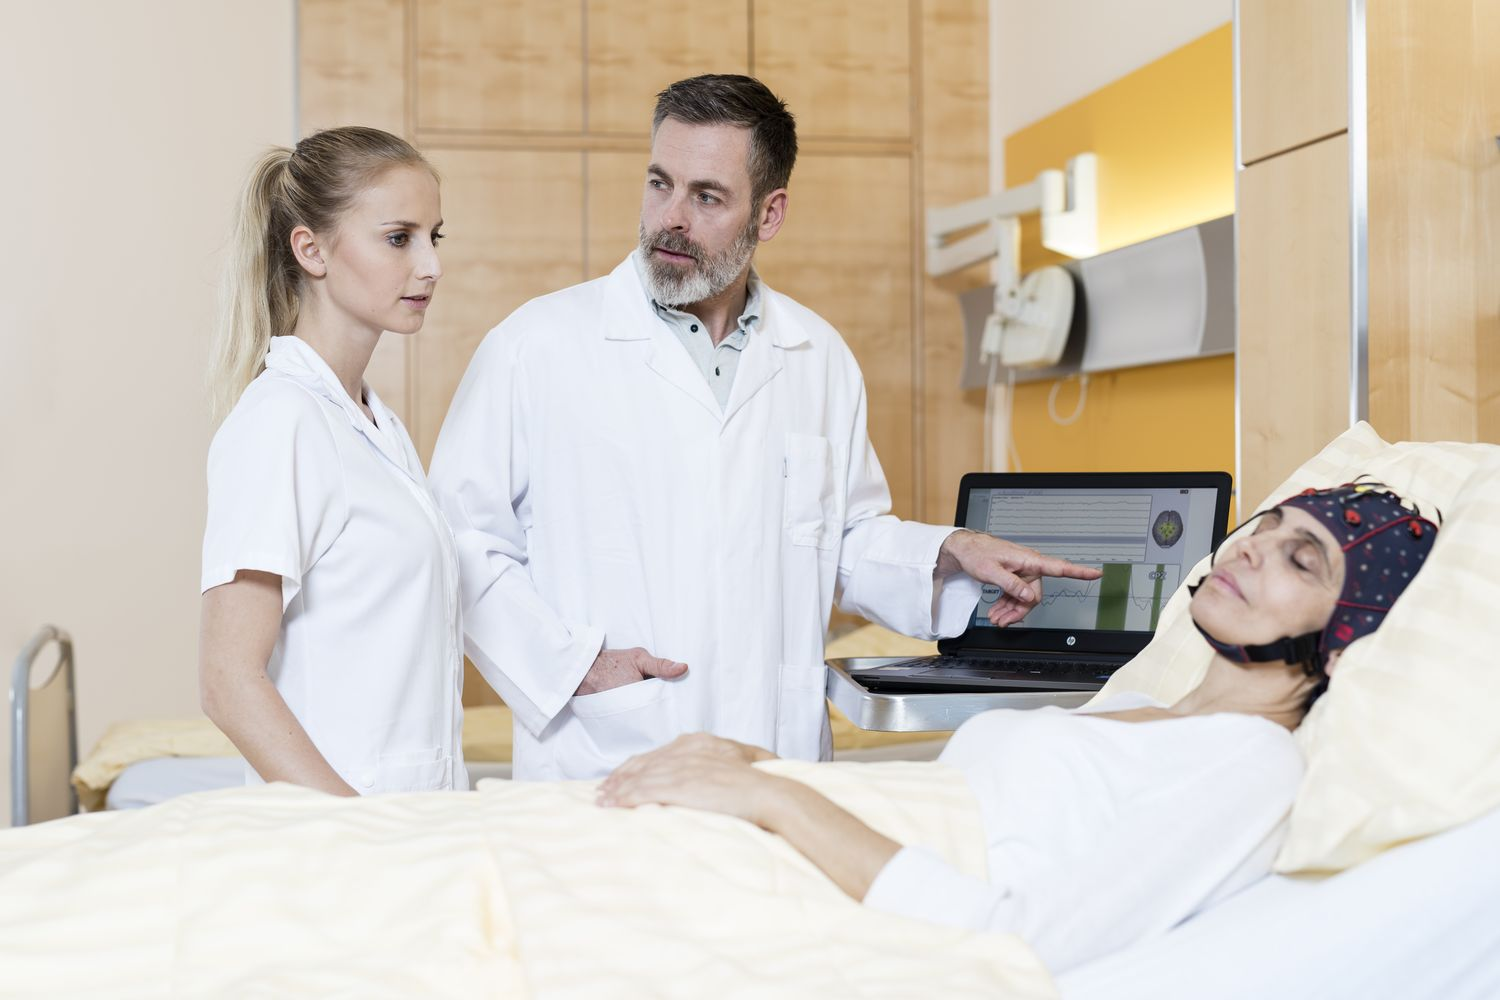
\includegraphics[height=3.5cm,width=7cm]{images/DoC.jpg}
\label{fig:digitalelectroencephalograph}
\end{figure}
\end{center}
\end{frame}

% Enfatizar que los paradigmas leen los estados mentales
\begin{frame}
\frametitle{Brain Computer Interfaces - System Components}
\begin{center}
\begin{figure}[]
\centering
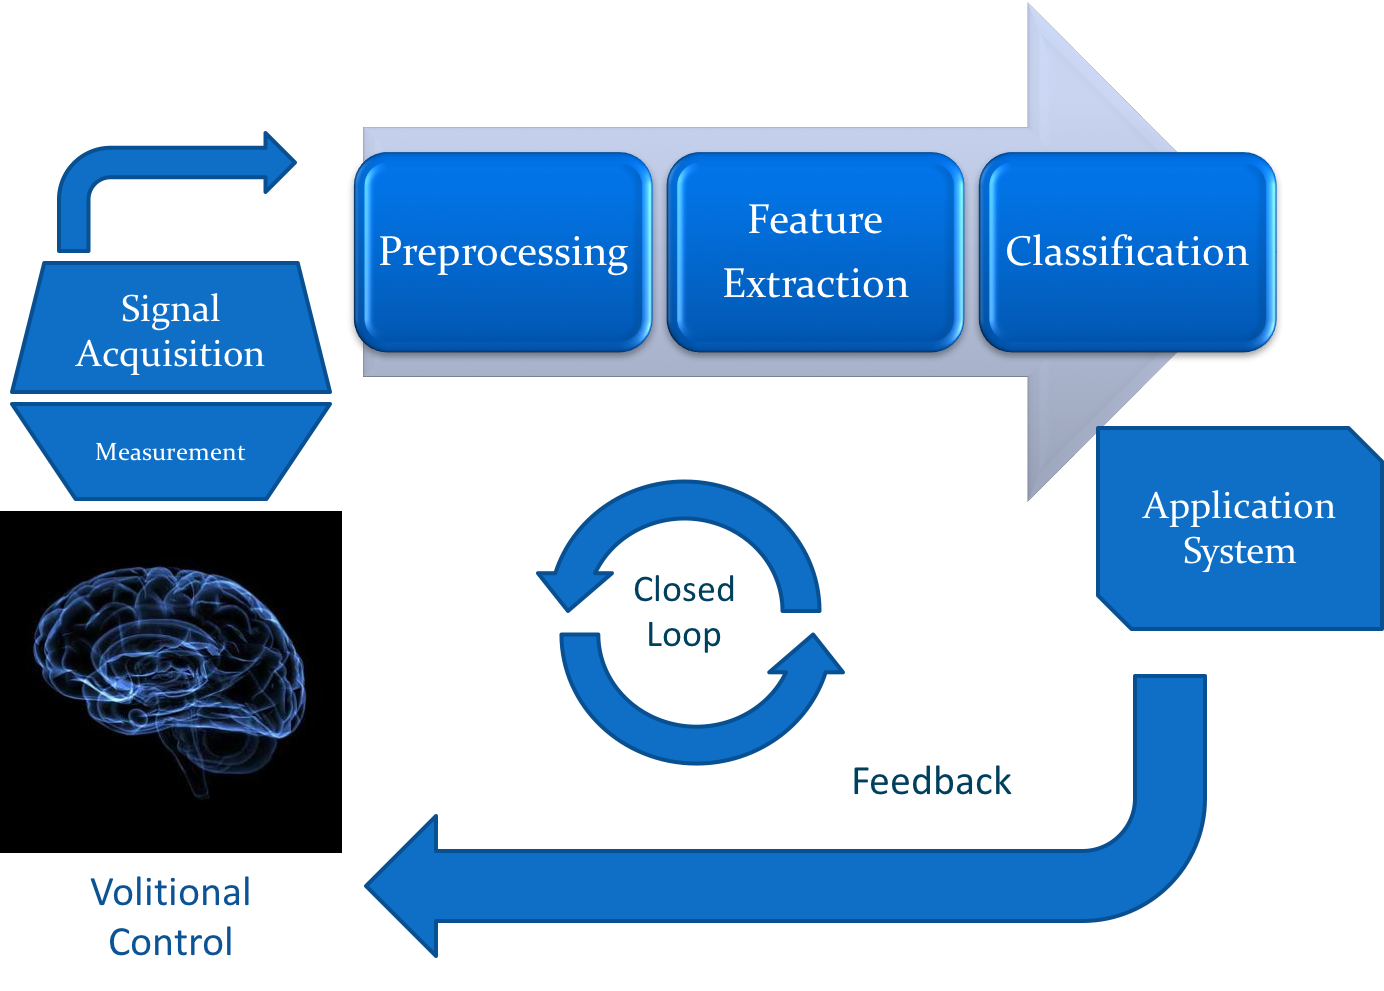
\includegraphics[scale=0.4]{images/bcichart.png}
\label{fig:bciblockdiagram}
\end{figure}
\end{center}
\end{frame}

\begin{frame}   
\frametitle{Brain Computer Interfaces - BCI Paradigms}
\begin{figure}[]
\centering
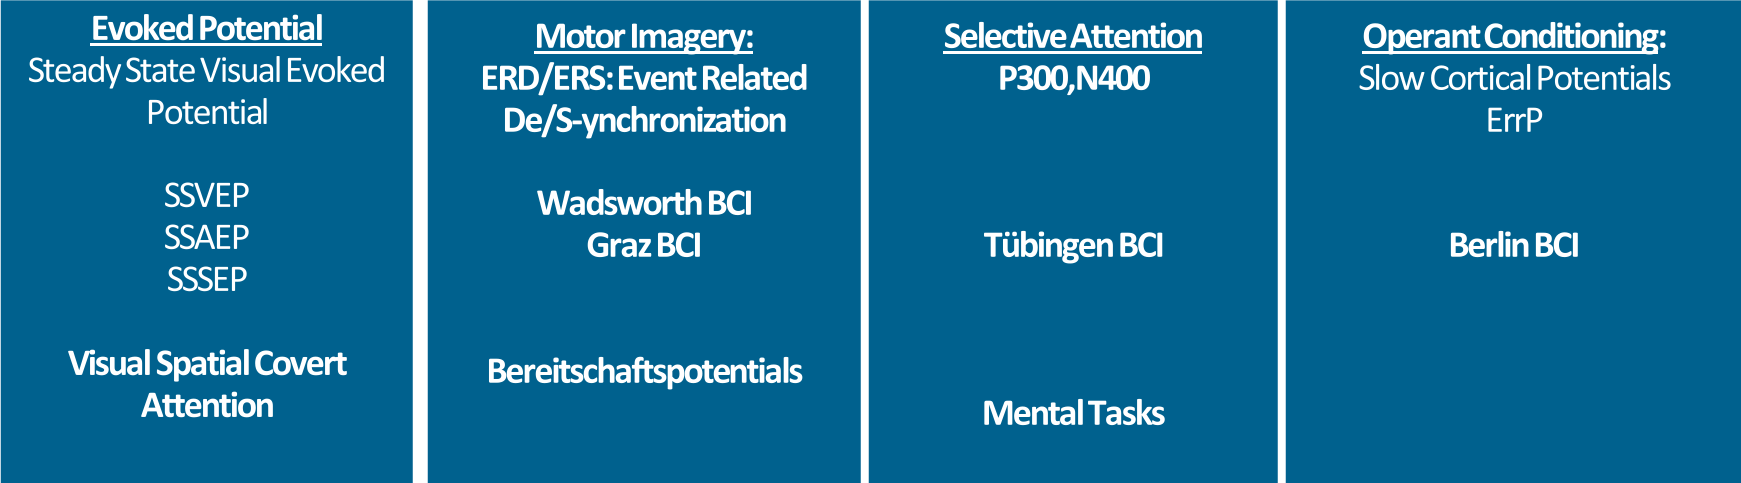
\includegraphics[scale=0.5]{images/BCIParadigms.png}
\label{fig:digitalelectroencephalograph}
\end{figure}
\end{frame}   
    

    \begin{frame}
        \frametitle{Brain Computer Interfaces - Problem Statement}
        \begin{center}
            \begin{itemize}
                \item<1-> \Fontre Clinical and Physician involvement~\footfullcite{Yuste2017}
                \item<2-> \Fontre Practical, relevant, and invariant features that convey good-enough information~\footfullcite{Perdikis2014}.
            \end{itemize}
        \end{center}
    \end{frame} 
    
    \section{Motivation}
    \begin{frame}
        \frametitle{Motivation}
        \begin{center}
                \LARGE Is it possible to analyze and discriminate electroencephalographic signals by automatic processing the shape of the waveforms using the \\ Histogram of Gradient Orientations ?
        \end{center}
    \end{frame}
    \begin{frame}
    
\frametitle{What we aim to do}
\begin{center}
\begin{enumerate}
\item<1-> \Fontre Construct analyzable 2D-image plots.
\item<2-> \Fontre Adaptation of the SIFT method to EEG time-series
\item<3-> \Fontre Feature extraction procedure
\item<4-> \Fontre Classification algorithm
\end{enumerate}
\end{center}
\end{frame}
    
\begin{frame}
\frametitle{Electroencephalography}
\begin{center}
\begin{figure}[]
\centering
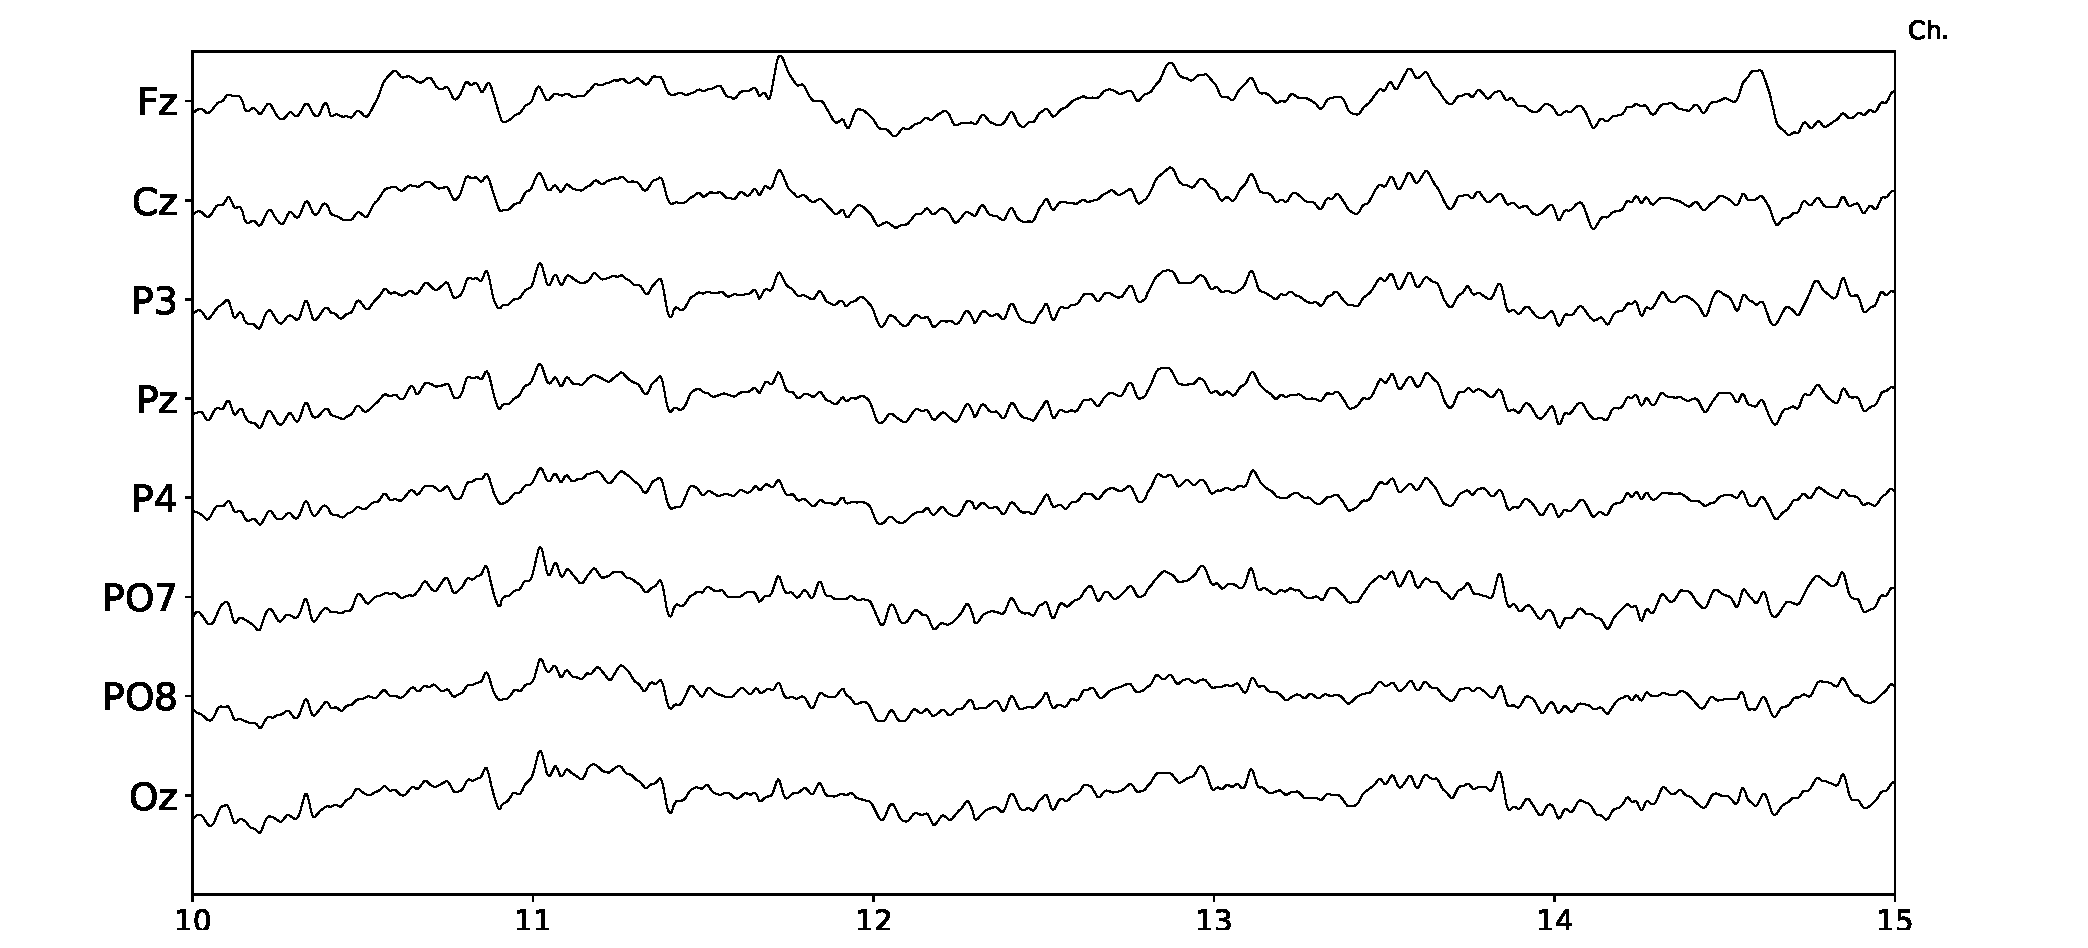
\includegraphics[height=6.0cm,width=14cm]{images/sampleeeg.eps}
\caption{Sample 8-channel EEG signal obtained from (g.Nautilus, g.Tec, Austria). Voltage in $\mu V$ vs time in seconds. Five seconds are displayed.}
\label{fig:sampleeeg}
\end{figure}
\end{center}
\end{frame}

\begin{frame}
\frametitle{Waveform-Based Algorithms}
\begin{center}
\begin{itemize}
 \item<1-> \Fontre Peak Picking/aEEG/Period Amplitude Analysis
 \item<1-> \Fontre Merge of Increasing and Decreasing Sequences
 \item<2-> \Fontre Permutation Entropy - PE
 \item<3-> \Fontre Matching Pursuit - MP
 \item<4-> \Fontre Slope Horizontal Chain Code - SHCC
\end{itemize}
\end{center}
\end{frame}


\section{The Histogram of Gradient Orientations}    
\begin{frame}
\frametitle{The Histogram of Gradient Orientations}
\begin{center}
\LARGE Proposal \\ The Histogram of Gradient Orientation
\end{center}
\end{frame}


\begin{frame}
\frametitle{The Histogram of Gradient Orientations - Feature Extraction Algorithm}
\begin{center}
\begin{enumerate}
 \item<1-> \Fontre Signal Preprocessing
 \item<2-> \Fontre Signal Segmentation
 \item<3-> \Fontre Signal Plotting
 \item<4-> \Fontre Keypoint Localization
 \item<5-> \Fontre Calculation of the Histogram of Gradient Orientation
\end{enumerate}
\end{center}
\end{frame}

%\begin{frame}
%\frametitle{The Histogram of Gradient Orientations}
%\begin{center}
%\begin{equation}
%\mathcal{I}^{(c)}(z_1,z_2) = \left\{ \begin{array}{rl}
%255 & \text{if} \   z_1 = \gamma_{t} \  n \quad \text{and}  \quad z_2 = \left\lfloor \gamma \; \tilde{x}(n,c) \right\rceil + z(c) \\
%0   & \mbox{otherwise}
%\end{array}\right.
%\label{eq:images}
%\end{equation}
%\noindent  where  $1 \leq c \leq C$ and $1 \leq n \leq N$. The amplitude scale factor $\gls{gamma}$ and time scale factor $\gls{gammat}$ are used to determine the image size and at the same time the image resolution. This scheme produces a black-and-white plot of the signal with $255$ being white and $0$ black.  There is one image per channel per segment. 
%\end{center}
%\end{frame}

\begin{frame}
\frametitle{Image Coordinate System}
\begin{center}
\begin{figure}[h!]
\centering
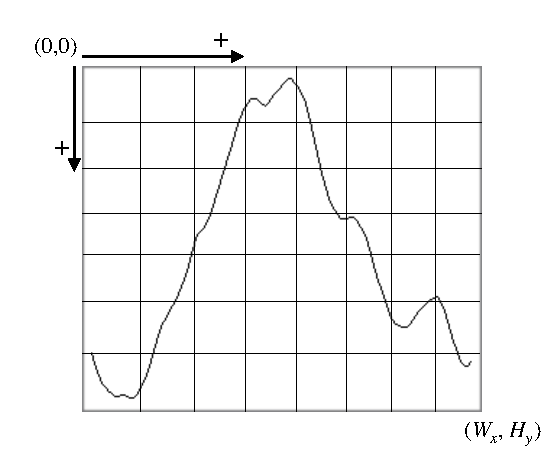
\includegraphics[scale=0.9]{images/imagecoordinatesystemresume.pdf}
\label{fig:imagecoordinatesystem}
\end{figure}
\end{center}
\end{frame}


\begin{frame}
\frametitle{Signal Plotting}
\begin{center}
\begin{figure}[h!]
\centering
\setlength\fboxsep{0pt}
\setlength\fboxrule{0.5pt}
\fbox{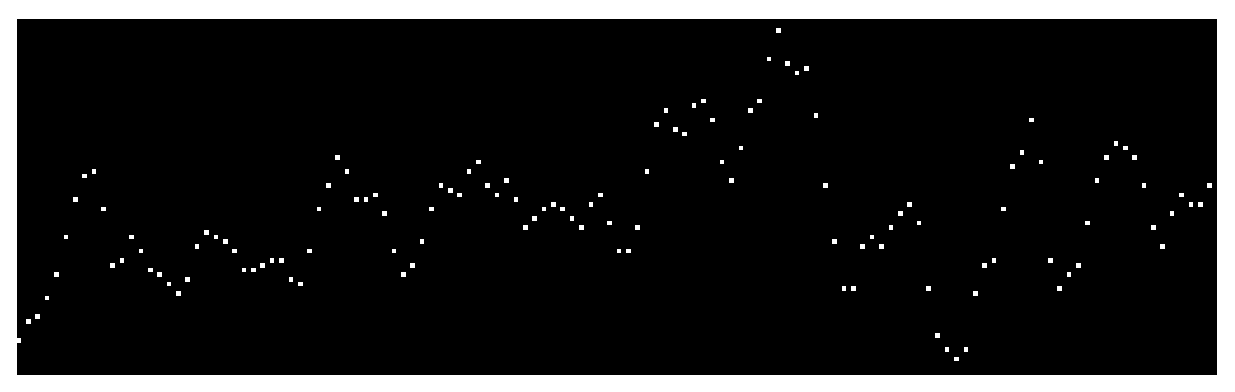
\includegraphics[height=2cm,width=7cm]{images/samplepoints.eps}}
\fbox{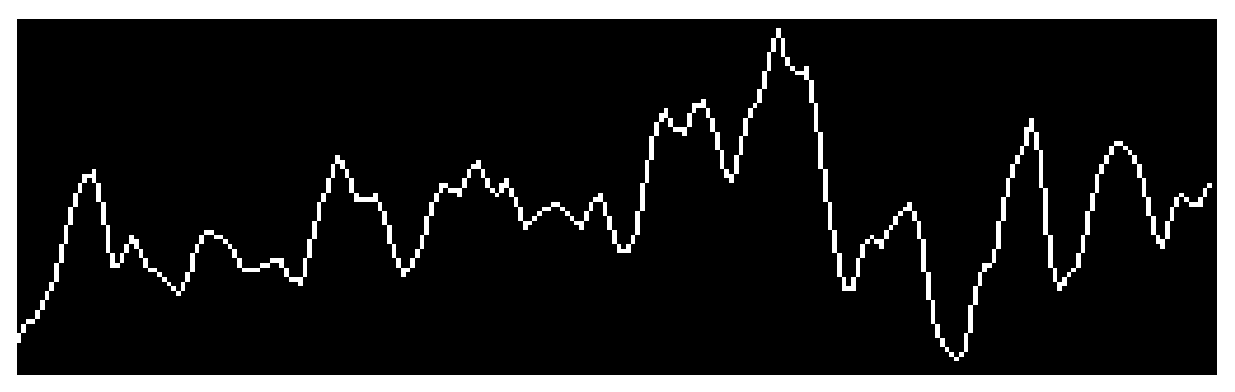
\includegraphics[height=2cm,width=7cm]{images/bresenham.eps}}\\
\fbox{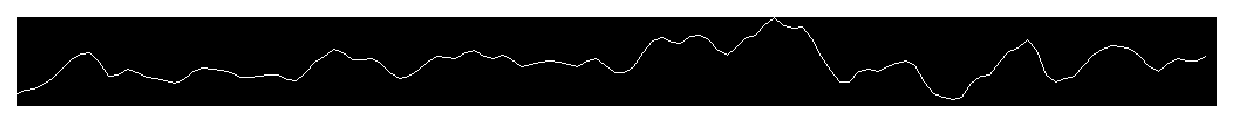
\includegraphics[height=2cm,width=7cm]{images/upscaled.eps}}
\fbox{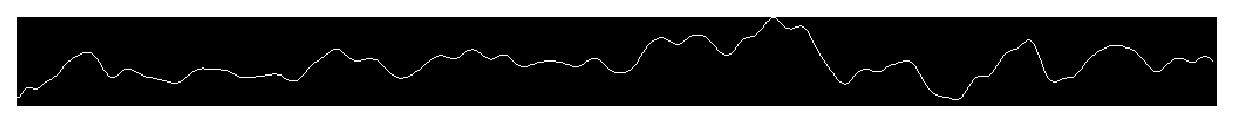
\includegraphics[height=2cm,width=7cm]{images/upsample.eps}}
\caption{Generated images based on different interpolation schemes.}
\label{fig:interpolation}
\end{figure}
\end{center}
\end{frame}



%\begin{frame}
%\frametitle{The Histogram of Gradient Orientations}
%\begin{center}
%\begin{figure}[htb]
%\centering
%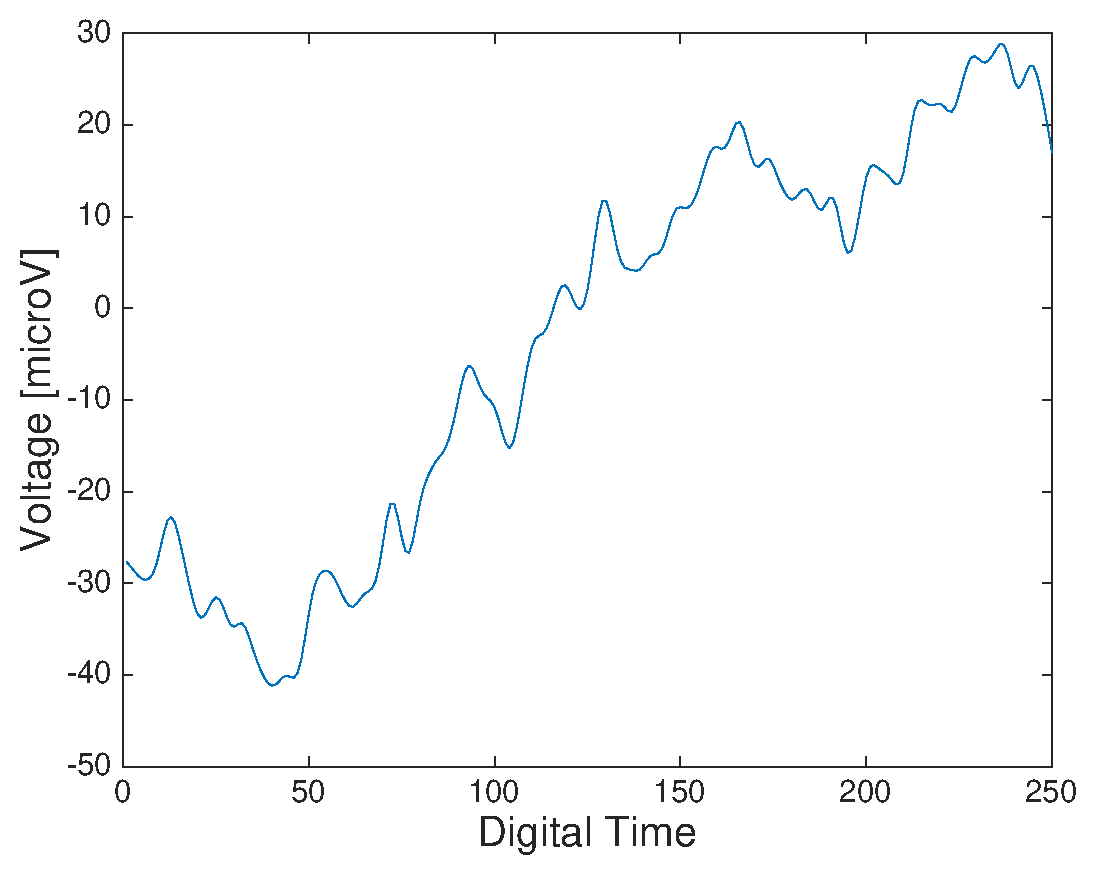
\includegraphics[height=5cm,width=5cm]{images/plotvsimage.eps}
%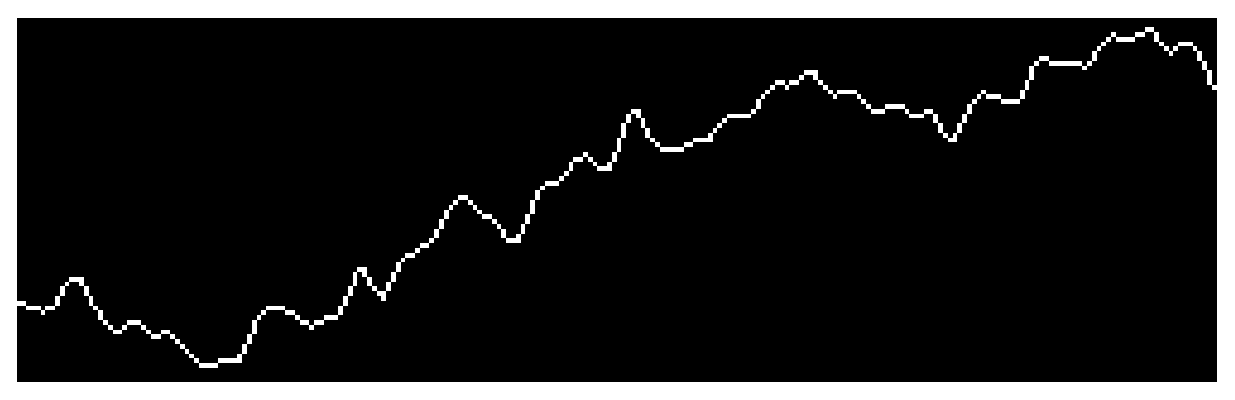
\includegraphics[height=5cm,width=10cm]{images/sampleplot.eps}
%\label{fig:plotvsimage}
%\end{figure}
%\end{center}
%\end{frame}

\begin{frame}
\frametitle{The Histogram of Gradient Orientations}
\begin{center}
\begin{figure}[h!]
\centering
\setlength\fboxsep{0pt}
\setlength\fboxrule{0.5pt}
\fbox{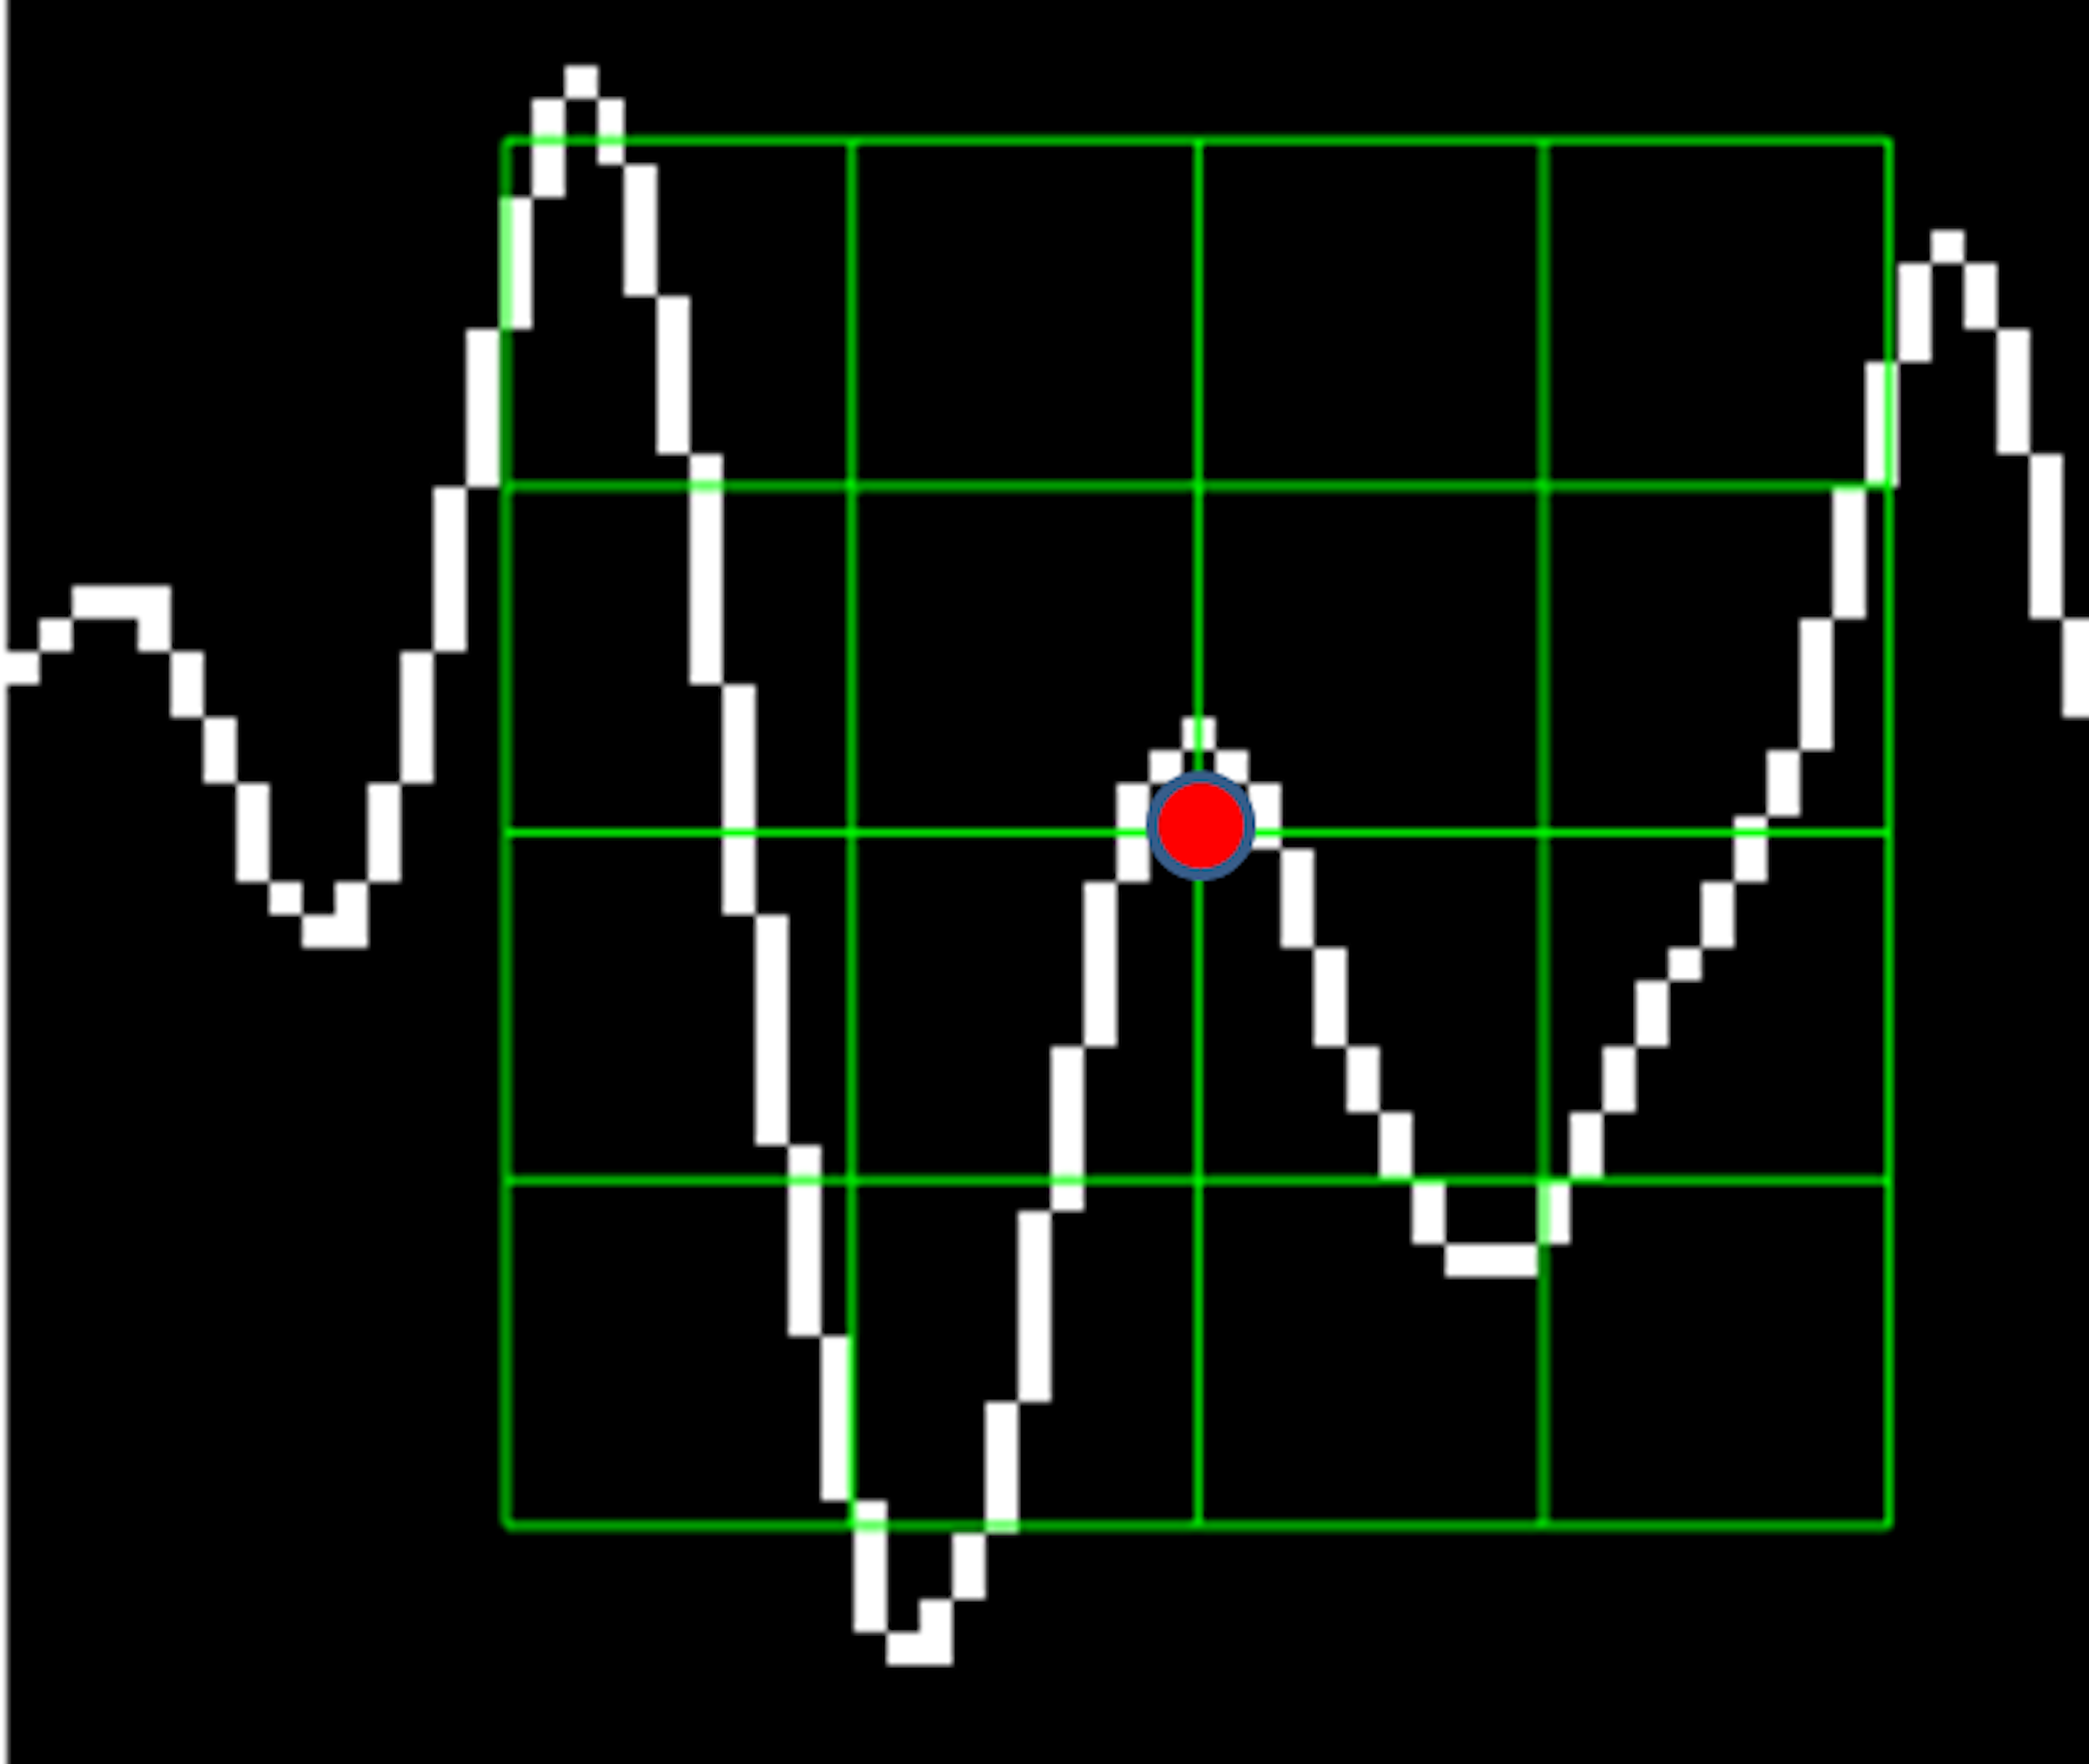
\includegraphics[width=7cm, height=2.5cm]{images/signalpatchkeypoint.png}}
\fbox{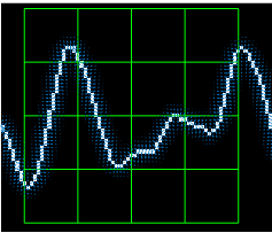
\includegraphics[width=7cm, height=2.5cm]{images/gradientsdescriptors.png}}\\
\fbox{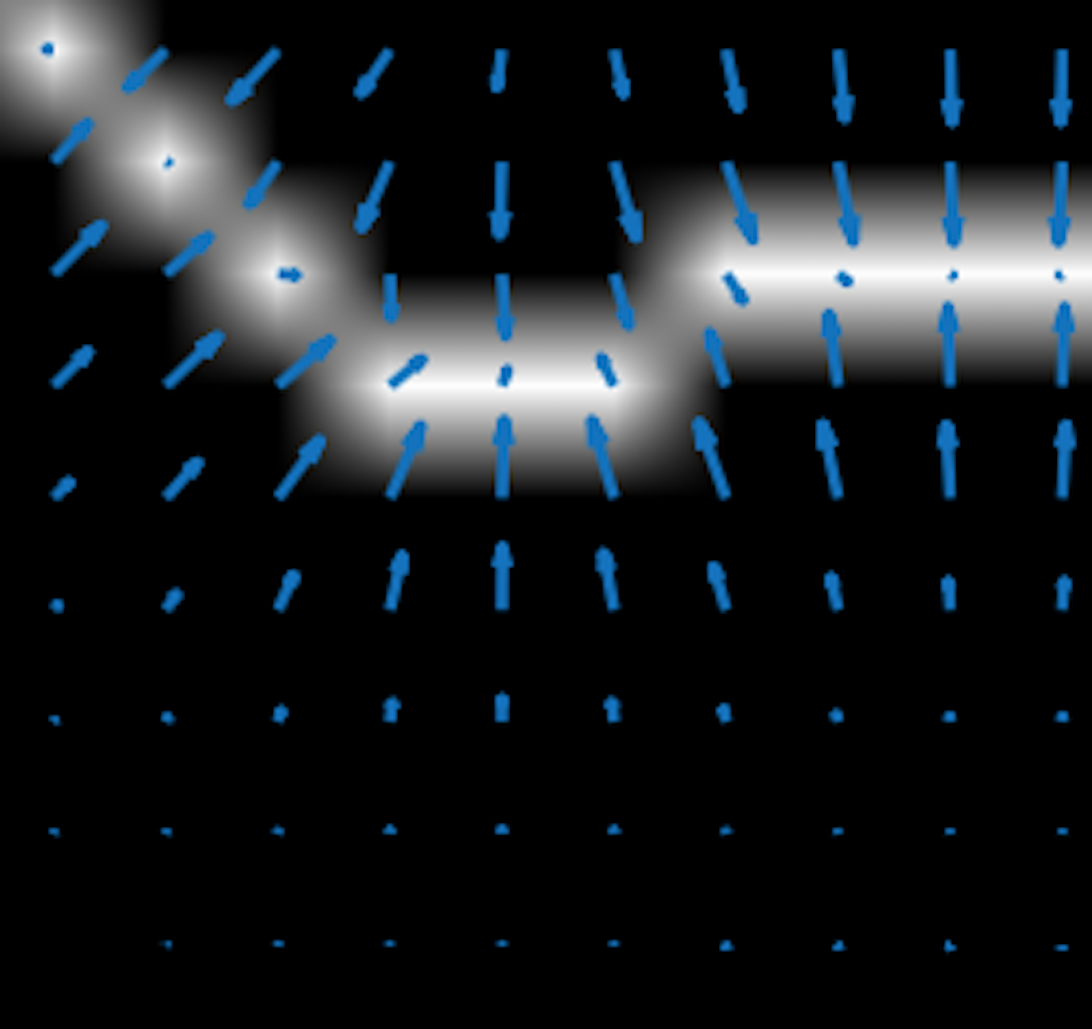
\includegraphics[width=7cm, height=2.5cm]{images/samplegradients.png}}
\fbox{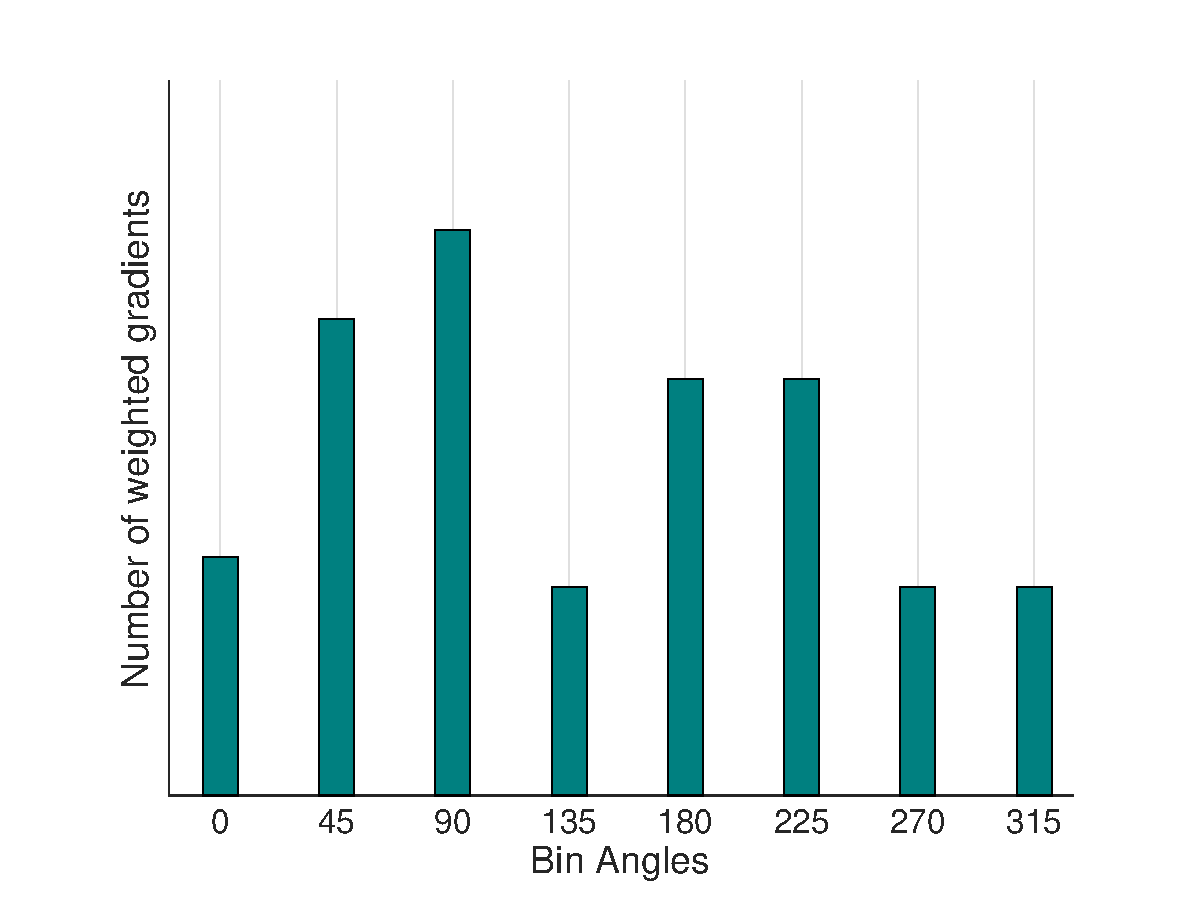
\includegraphics[width=7cm, height=2.5cm]{images/histogramchart.eps}}
\label{fig:sampledescriptor}
\end{figure}
\end{center}
\end{frame}


\begin{frame}
\frametitle{Keypoint Localization}
\begin{center}
\begin{figure}[h!]
\centering
\setlength\fboxsep{0pt}
\setlength\fboxrule{0.5pt}
\fbox{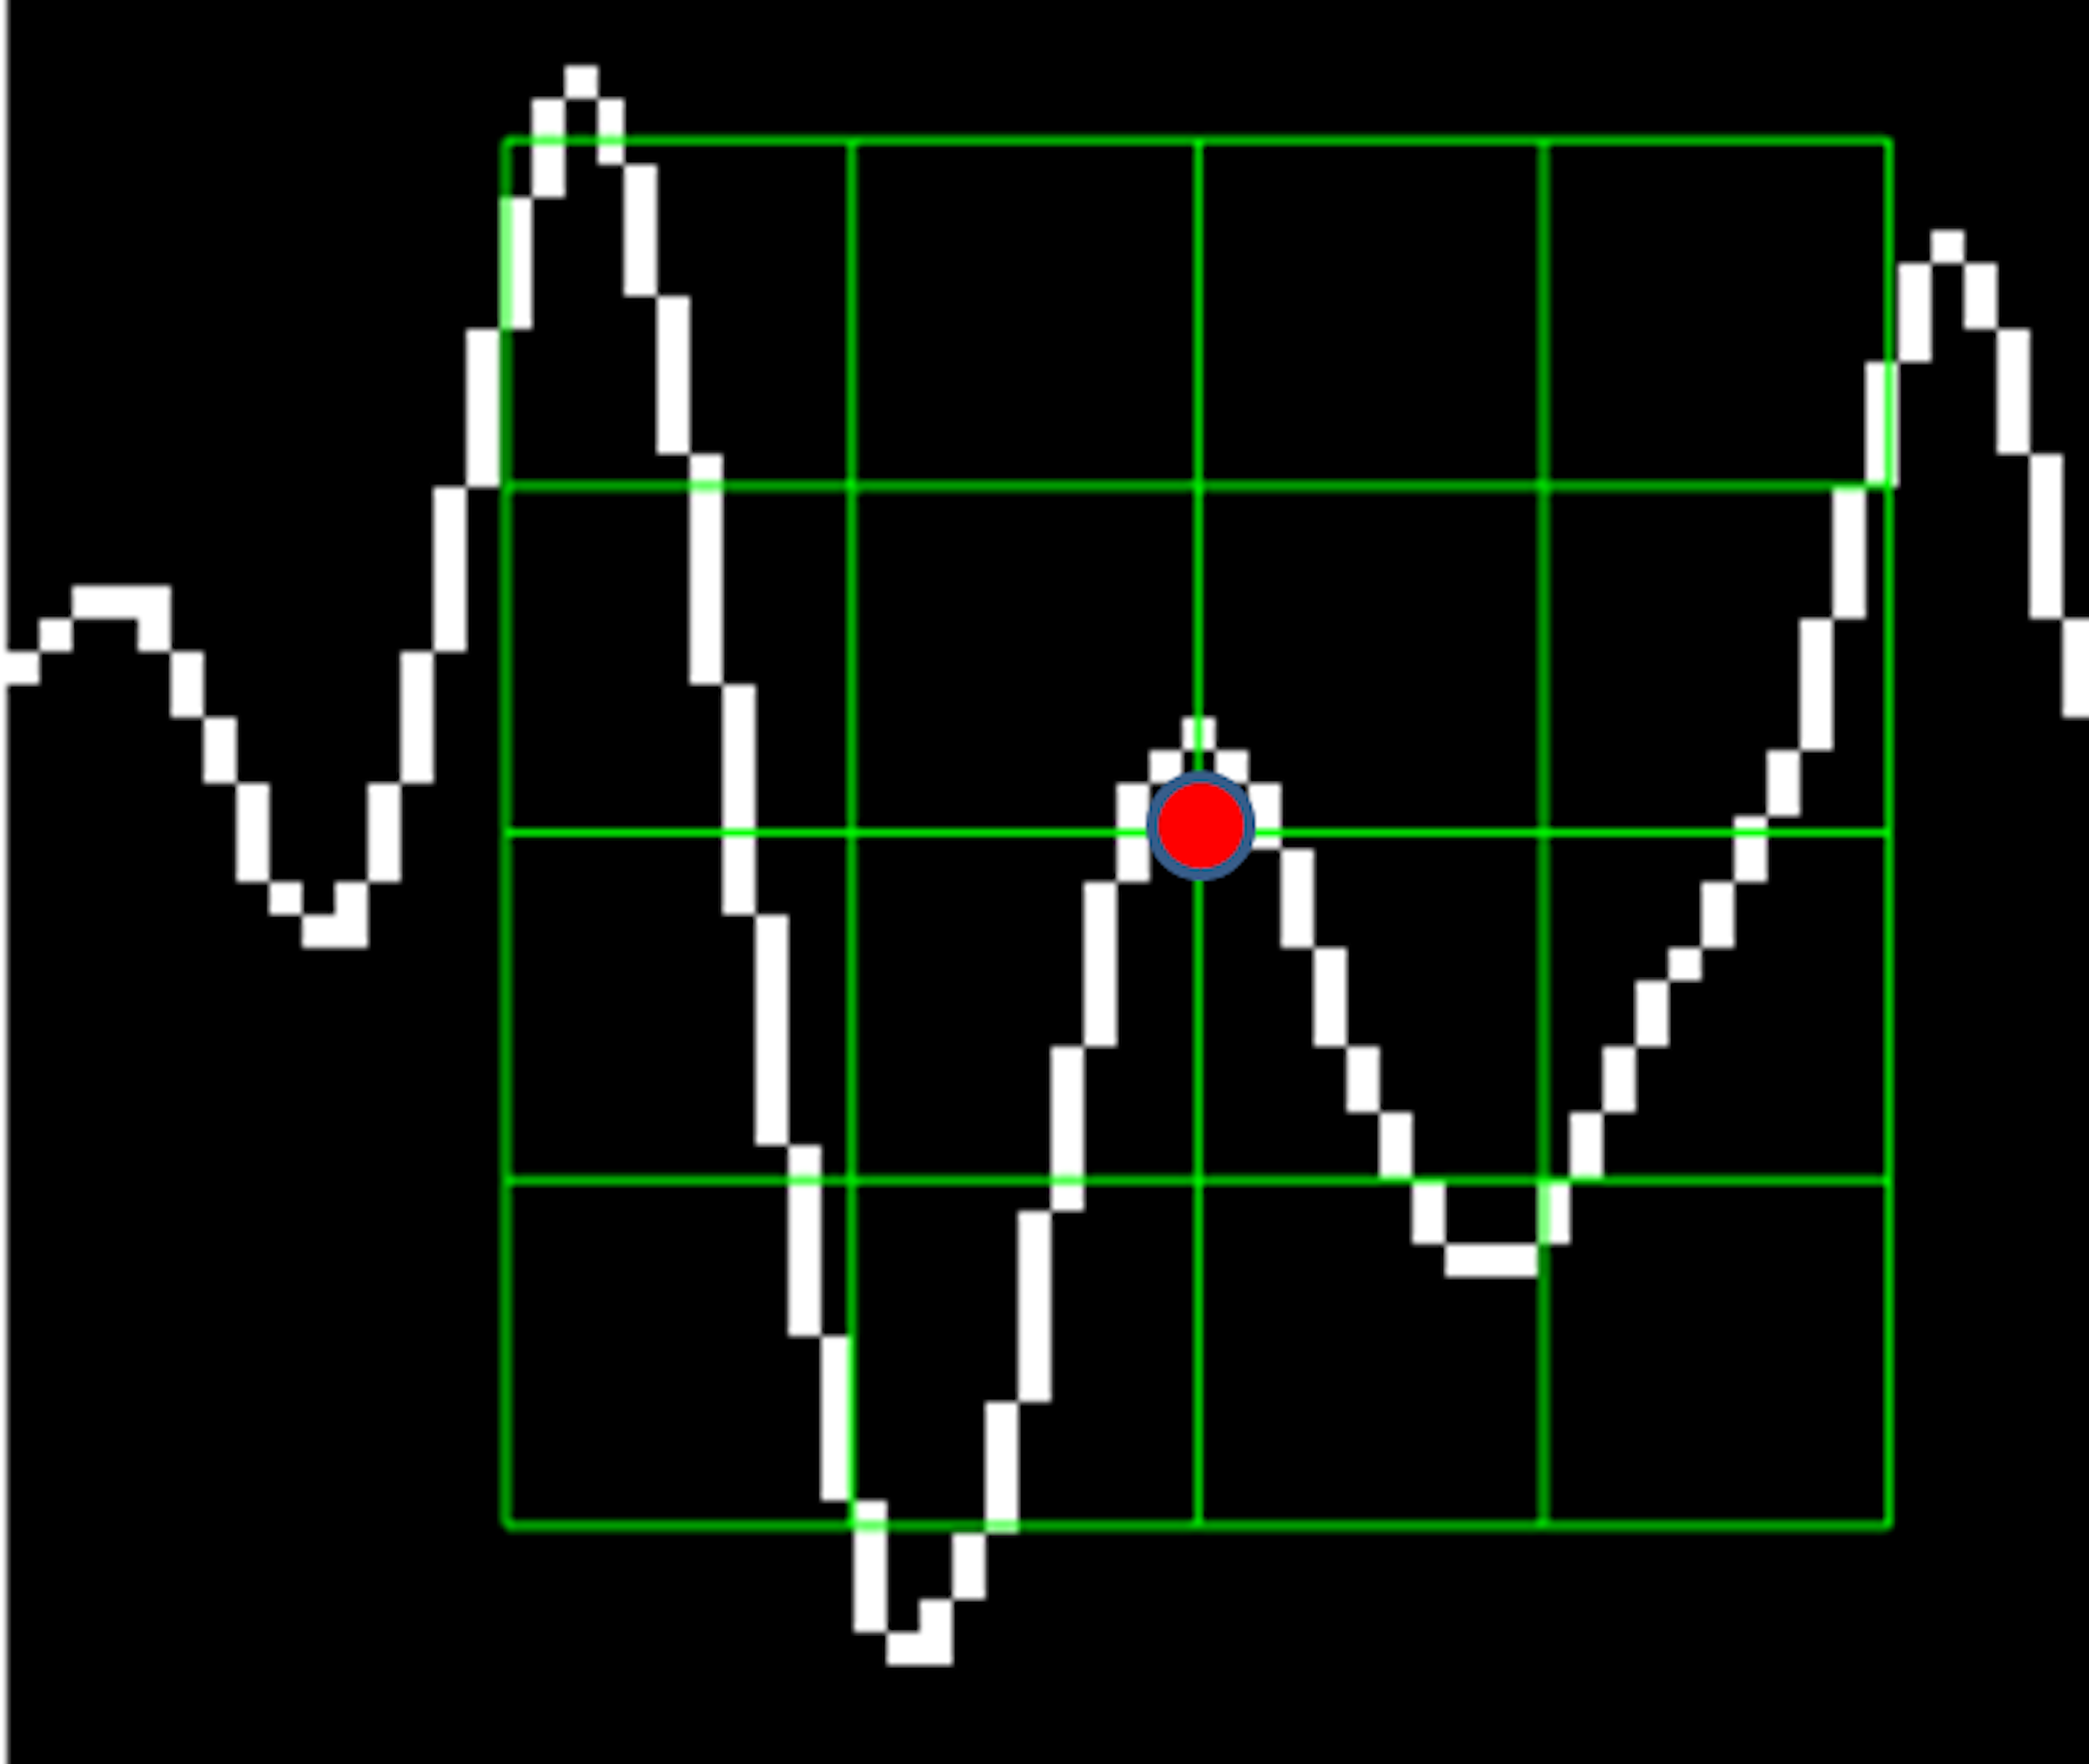
\includegraphics[width=14cm,height=6cm]{images/signalpatchkeypoint.png}}
\label{fig:sampledescriptor}
\end{figure}
\end{center}
\end{frame}

\begin{frame}
\frametitle{Pixel Gradient Vector Field}
\begin{center}
\begin{figure}[h!]
\centering
\setlength\fboxsep{0pt}
\setlength\fboxrule{0.5pt}
\fbox{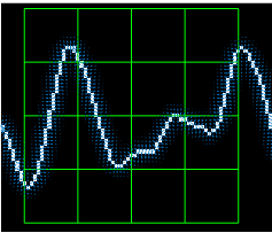
\includegraphics[width=14cm,height=6cm]{images/gradientsdescriptors.png}}
\label{fig:sampledescriptor}
\end{figure}
\end{center}
\end{frame}

\begin{frame}
\frametitle{Pixel Gradient Vector Field}
\begin{center}
\begin{figure}[h!]
\centering
\setlength\fboxsep{0pt}
\setlength\fboxrule{0.5pt}
\fbox{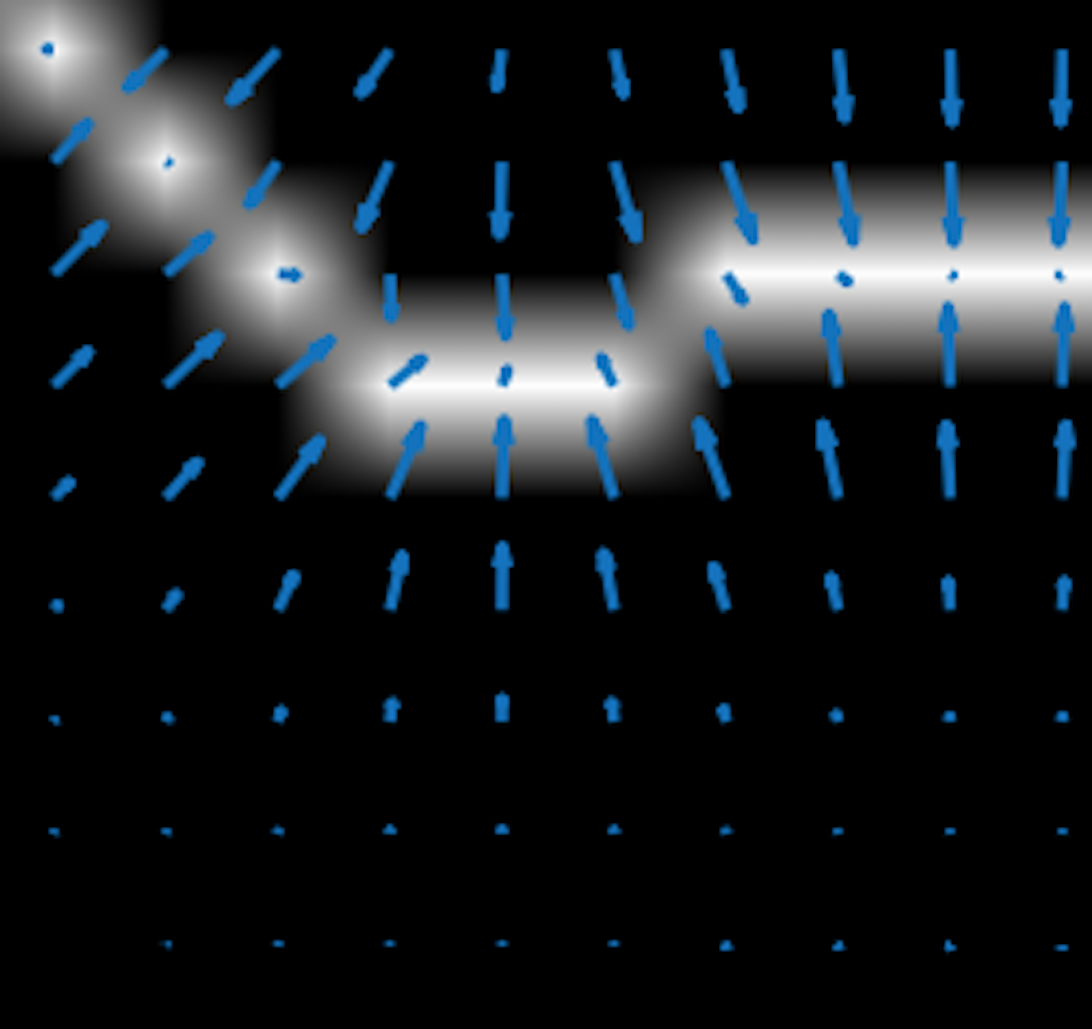
\includegraphics[width=14cm,height=6cm]{images/samplegradients.png}}
\label{fig:sampledescriptor}
\end{figure}
\end{center}
\end{frame}

\begin{frame}
\frametitle{Orientation histogram}
\begin{center}
\begin{figure}[h!]
\centering
\setlength\fboxsep{0pt}
\setlength\fboxrule{0.5pt}
\fbox{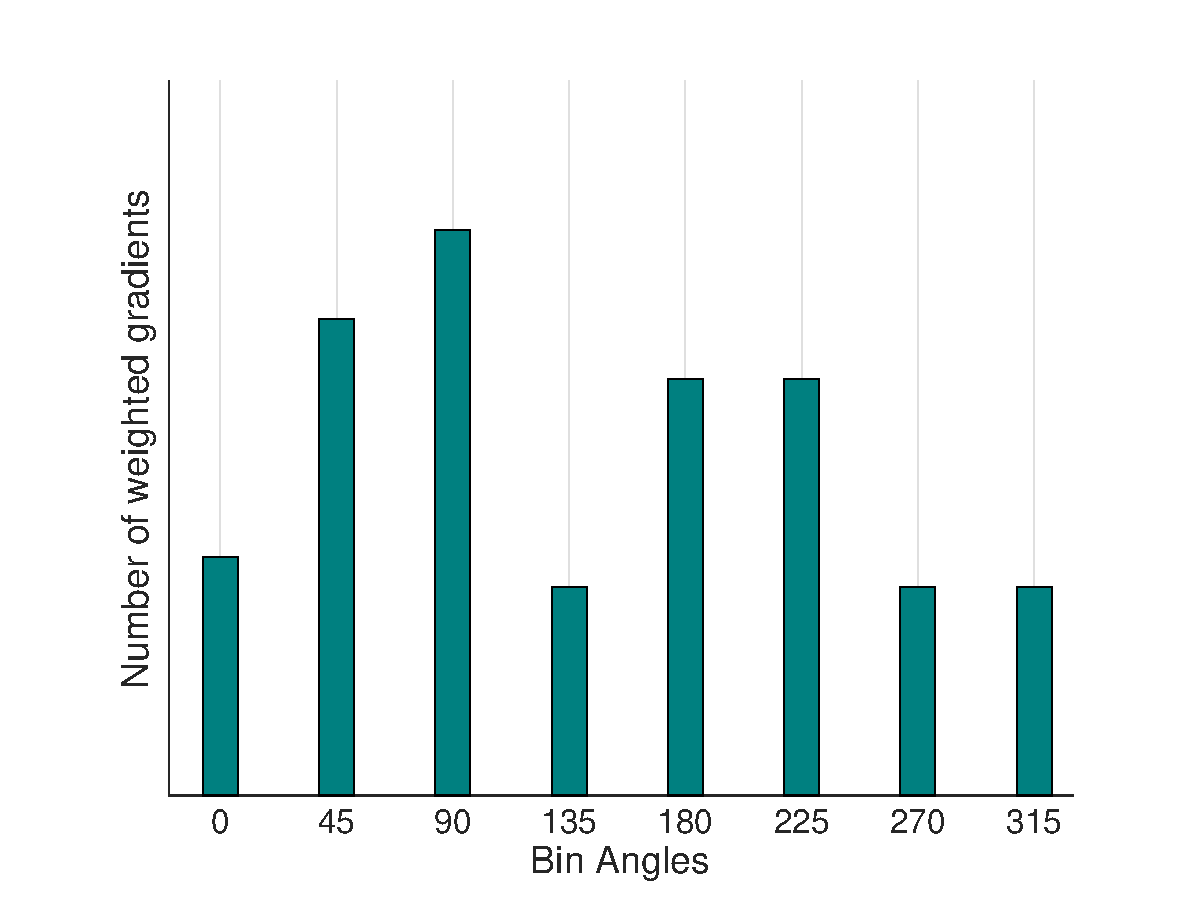
\includegraphics[width=10cm,height=6cm ]{images/histogramchart.eps}}
\label{fig:sampledescriptor}
\end{figure}
\end{center}
\end{frame}

\begin{frame}
\frametitle{Histogram Calculation}
\begin{center}

\begin{equation}
 h(\theta,i,j) = \sum_{\mathbf{p}} \omega_\mathrm{ang}(\angle J(\mathbf{p}) - \theta)\, \omega_{ij}\left(\mathbf{p} - \mathbf{kp} \right)\, \left\lVert J(\mathbf{p})\right\rVert 
\label{eq:histogram}
\end{equation}

\begin{itemize}
\item $\theta$ is the angle bin with $ \theta \in \{0, 45, 90, 135, 180, 225, 270, 315\} $.
\item $ i,j = \{0,1,2,3\} $ indexes of the 16 grid blocks.
\item $\mathbf{kp}$ is the keypoint center location.
\item $\mathbf{p}$ is a pixel from within the patch, centered around $\mathbf{kp}$.
\item $\angle J(\mathbf{p}) $ is the angle of the gradient vector.
\item $ \left\lVert J(\mathbf{p}) \right\rVert $ is the norm of the gradient vector in the pixel $\mathbf{p}$.
\item $\omega_\mathrm{ang}(\cdot) $ scalar and $ \omega_{ij}(\cdot) $ vector linear interpolation functions~\footfullcite{Lowe2004,Vedaldi2010}.
\end{itemize}

\end{center}
\end{frame}

\begin{frame}
\frametitle{Descriptor}
\begin{center}
\begin{figure}[h!]
\centering
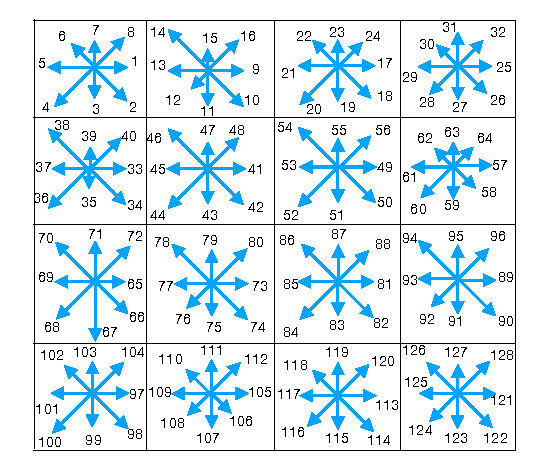
\includegraphics[scale=0.9]{images/gradientorientations.pdf}
\label{fig:orientationsfull}
\end{figure}
\end{center}
\end{frame}


\begin{frame}
\frametitle{Patch Geometry}
\begin{center}
\begin{figure}[h!]
\centering
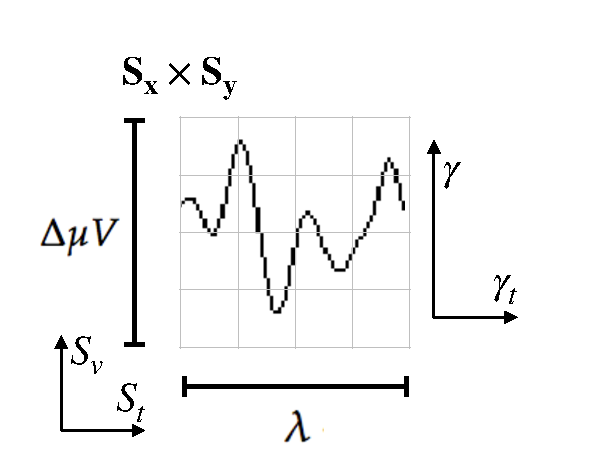
\includegraphics[scale=0.9]{images/patchgeometry.pdf}
\label{fig:patchgeometry}
\end{figure}
\end{center}
\end{frame}

\begin{frame}
\frametitle{Proposed Classification Method}
\begin{center}
\begin{equation}
\hat{L} = \arg \min_{L} \sum_{i=1}^{Q} \sum_{h=1}^{\gls{k}} {\left\lVert \mathbf{q}_{i}^{(bpc)} -  \mathbf{d}_{h}^{(L,bpc)} \right\rVert}  ^{2} 
\label{eq:classification}
\end{equation}
\begin{itemize}
\item $L$ class label.
\item $Q$ number of descriptors extracted from the query image. 
\item $\mathbf{q}_{i}^{(bpc)} $ query descriptors.
\item $\mathbf{d}_{h}^{(L,bpc)} $ neighbors descriptors from template dictionary of class $L$.
\item $\mathbf{d}_{h}^{(L,bpc)} \in N_T(  \mathbf{q}_{i}^{(bpc)} )$.
\item $N_T(  \mathbf{q}_{i}^{(bpc)} ) = \{ \mathbf{d}_{h}^{(bpc)} \in T_{L}^{bpc} / \mathbf{d} $ is the $\gls{k}$-nearest neighbor of $  \mathbf{q}_{i}^{(bpc)} \}$.
\item $\hat{L}$ predicted class label.
\item $\gls{k}$ the number of neighbors to pick from the template~\footfullcite{Boiman2008}.
\end{itemize}
\end{center}
\end{frame}

\begin{frame}
\frametitle{Classification Algorithm}
\begin{center}
\begin{figure}[h!]
\centering
\includegraphics[height=7.5cm,width=13cm]{images/ClassificationFull.pdf}
\label{fig:nbnnclassification}
\end{figure}
\end{center}
\end{frame}   

\section{Experimental Validation}
\begin{frame}
\frametitle{Experimental Validation}
\begin{center}
\LARGE Experimental Validation
\end{center}
\end{frame}

\begin{frame}
\frametitle{Experimental Validation}
\begin{center}
\begin{itemize}
 \item<1-> \Fontre Alpha Waves Wiggles
 \item<2-> \Fontre $\mu$ Rhythm
 \item<3-> \Fontre The P300 Waveform
\end{itemize}
\end{center}
\end{frame}     

\begin{frame}
\frametitle{Experimental Validation}
\begin{center}
\LARGE Alpha Waves wiggles
\end{center}
\end{frame}

\begin{frame}
\frametitle{Alpha Waves Datasets}
\begin{center}
\begin{itemize}
\item \Fontre Dataset I: EPOC Emotiv Consumer Grade EEG Device 
\begin{itemize}
\item 128 Hz, 14 channels, 10 subjects, 10 class 1 vs 10 class 2.
\end{itemize}
\item \Fontre Dataset II: EEG MI NHS PhysioNet
\begin{itemize}
\item 160 Hz, 64 channels, 25 subjects, Run 1 vs Run 2, 60 vs 60.
\end{itemize}
\end{itemize}
\end{center}
\end{frame}

\begin{frame}   
\frametitle{EEG Consumer Grade Digital Device and EEG Signals}
\begin{figure}[]
\centering
\begin{columns}
\begin{column}{0.5\textwidth}
\setlength\fboxsep{0pt}
\setlength\fboxrule{0.5pt}
\fbox{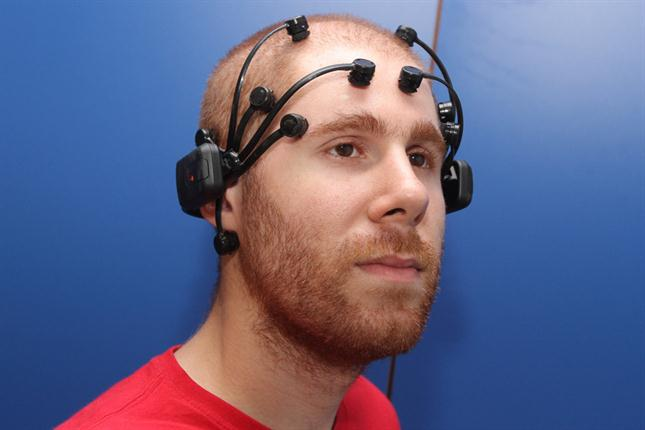
\includegraphics[height=7cm,width=7.8cm]{images/emotivsubject.jpg}}
\end{column}
\begin{column}{0.5\textwidth}
\setlength\fboxsep{0pt}
\setlength\fboxrule{0.5pt}
\fbox{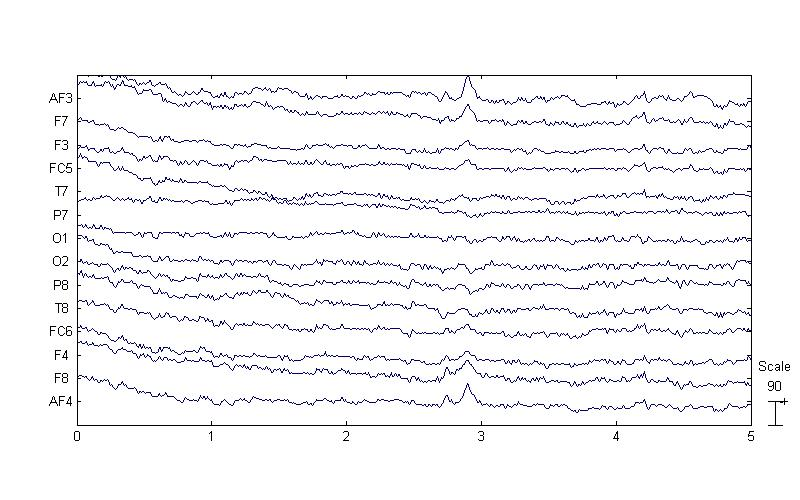
\includegraphics[height=3.5cm,width=8cm]{images/eeglab1.jpg}}
\fbox{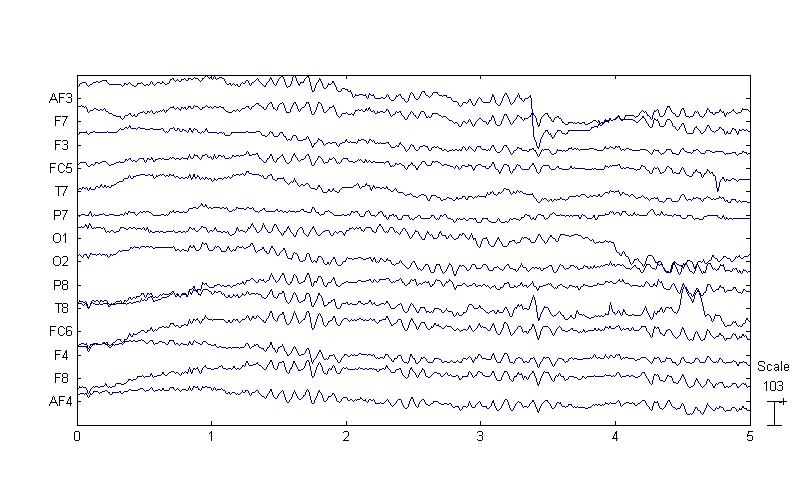
\includegraphics[height=3.5cm,width=8cm]{images/eeglab2.jpg}}
\end{column}
\end{columns}
\caption{EPOC Emotiv and Alpha Waves signals}
\label{fig:digitalelectroencephalograph}
\end{figure}
\end{frame}

\begin{frame}   
\frametitle{Keypoint populations}
\begin{figure}[]
\centering
\fbox{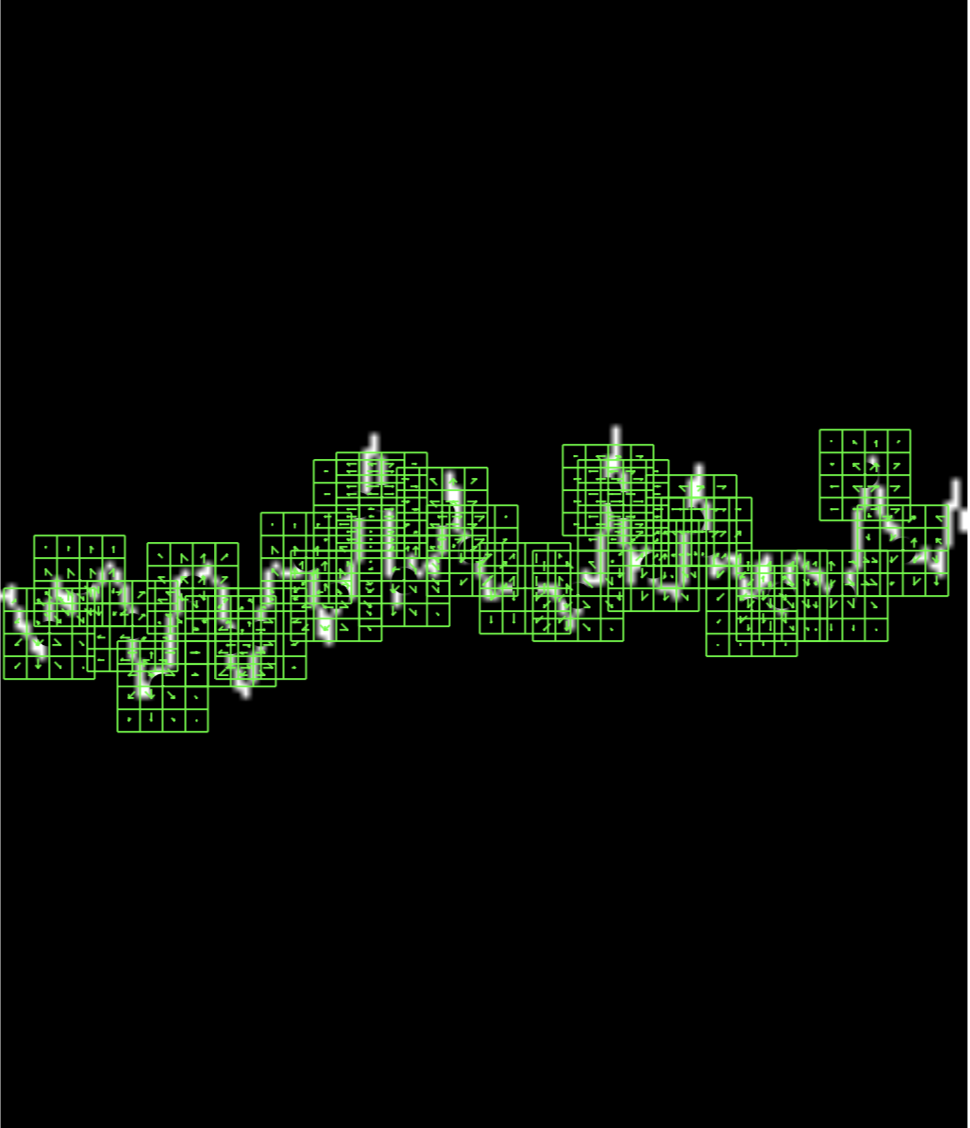
\includegraphics[width=7.5cm, height=7cm]{images/SignalWithFullDescriptors3.png}}
\label{fig:digitalelectroencephalograph}
\end{figure}
\end{frame}


\begin{frame}
\frametitle{10-Fold Cross Validated Binary Classification Accuracy - Dataset I}
\begin{figure}[h!]
\centering
%\subfigure[Ten-fold cross-validated accuracy values, averaged across $10$ subjects.  Descriptors used for calibration are intermixed to create one template dictionary which is used for all subjects.]
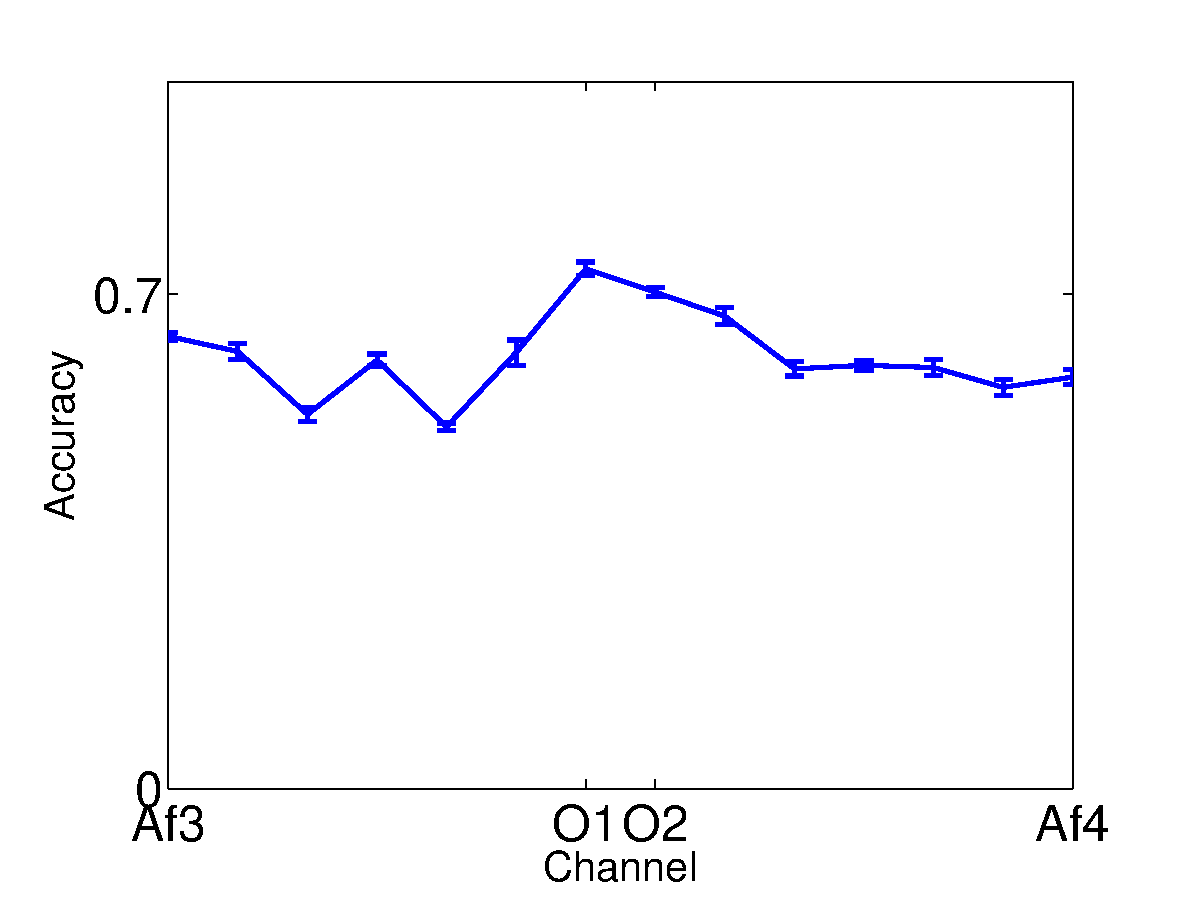
\includegraphics[width=7.5cm, height=5cm]{images/Dataset1AccuracyPerChannel}
%\subfigure[Amplified image containing a sample patch located on one of the images generated for one 1-second long segment of this dataset. The keypoint location is on a sample point along the EEG trace.]
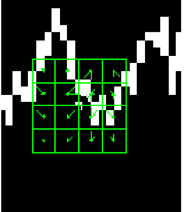
\includegraphics[width=7.5cm, height=5cm]{images/AlphaWaveSampleEEG.png}
\caption{The horizontal patch scale $\gls{St}$ and the vertical patch scale $\gls{Sv}$ are set to $1$, whereas $\gls{gamma}$ and $\gls{gammat}$ are set to $2$, which corresponds to a variation of $\gls{DeltamuV} = 10$ microvolts in the signal amplitude during $\gls{lambda}=0.08$ $\si{seconds}$.}
\label{fig:alpharesultsdataseti}
\end{figure}
\end{frame}

\begin{frame}
\frametitle{10-Fold Cross Validated Binary Classification Accuracy - Dataset II}
\begin{figure}[h!]
\centering
%\subfigure[Ten-fold cross-validated accuracies values for a randomly selected subject (number 12), using runs 1 and 2.]
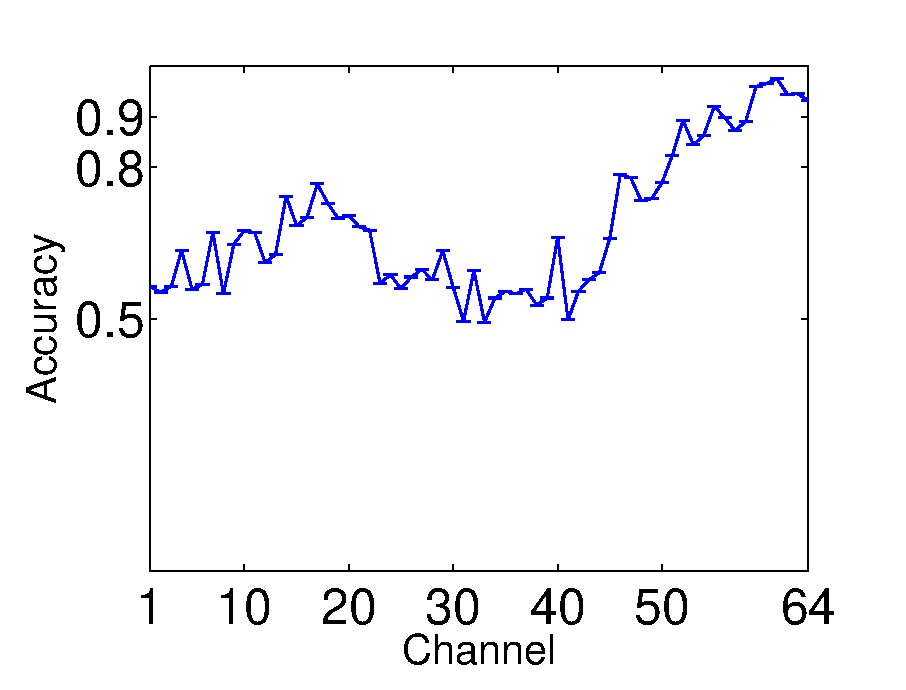
\includegraphics[width=7.5cm, height=5cm]{images/DatasetPhysionetAccuracyPerChannel}
%\subfigure[Ten-fold cross-validated accuracy boxplots for occipital channels O1, Oz, O2 and Iz, for the 25 subjects. Mean values are around $70\%$.]
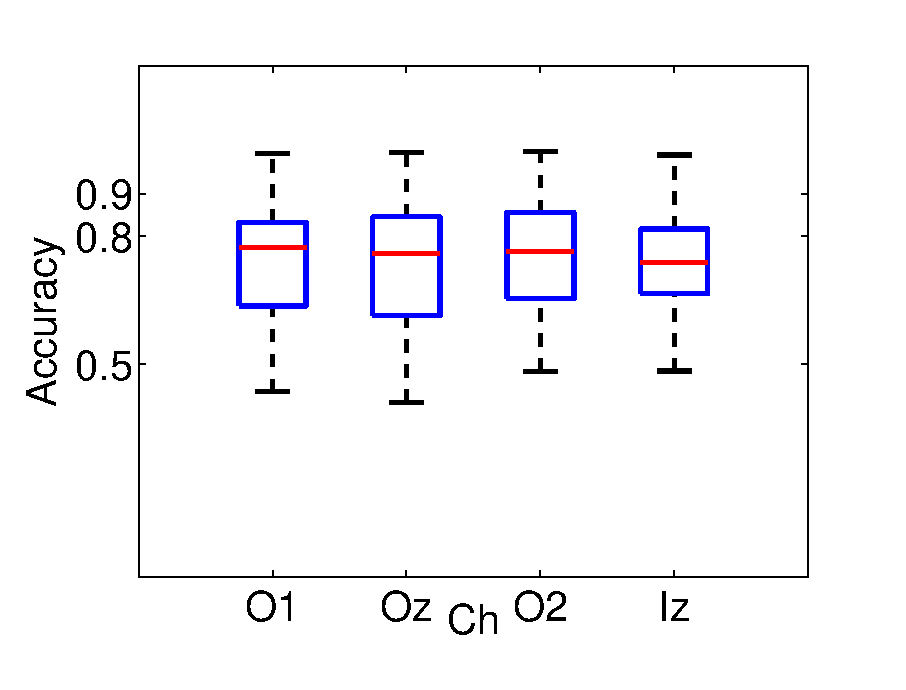
\includegraphics[width=7.5cm, height=5cm]{images/DatasetPhysionetBoxPlots}
\caption{Binary classification accuracy for subject 25 and boxplots obtained for the 25 subjects on 4 occipital channels}.
\label{fig:alpharesultsdatasetii}
\end{figure}
\end{frame}

\begin{frame}
\frametitle{Experimental Validation}
\begin{center}
\LARGE $\mu$ Rhythm
\end{center}
\end{frame}

\begin{frame}
\frametitle{Dataset 002-2014 BNCI-Horizon 2020 (Steyrl, Scherer et al 2015)}
\begin{figure}[thpb]
\centering
\setlength\fboxsep{0pt}
\setlength\fboxrule{0.5pt}
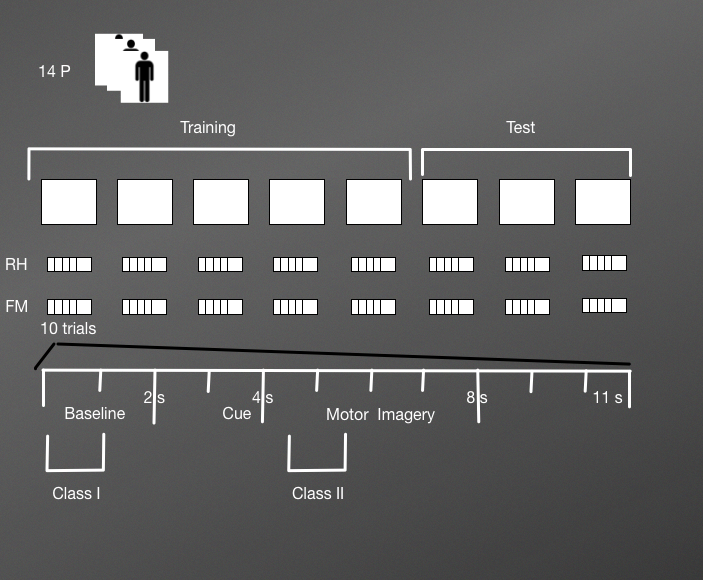
\includegraphics[scale=0.34]{images/DatasetIIIDiagram2}    
\end{figure} 	
\end{frame}	

   \begin{frame}   
   \frametitle{$\mu$ Rhythm}
   \begin{figure}[thpb]
      \centering
      \setlength\fboxsep{0pt}
	  \setlength\fboxrule{0.5pt}
       \fbox{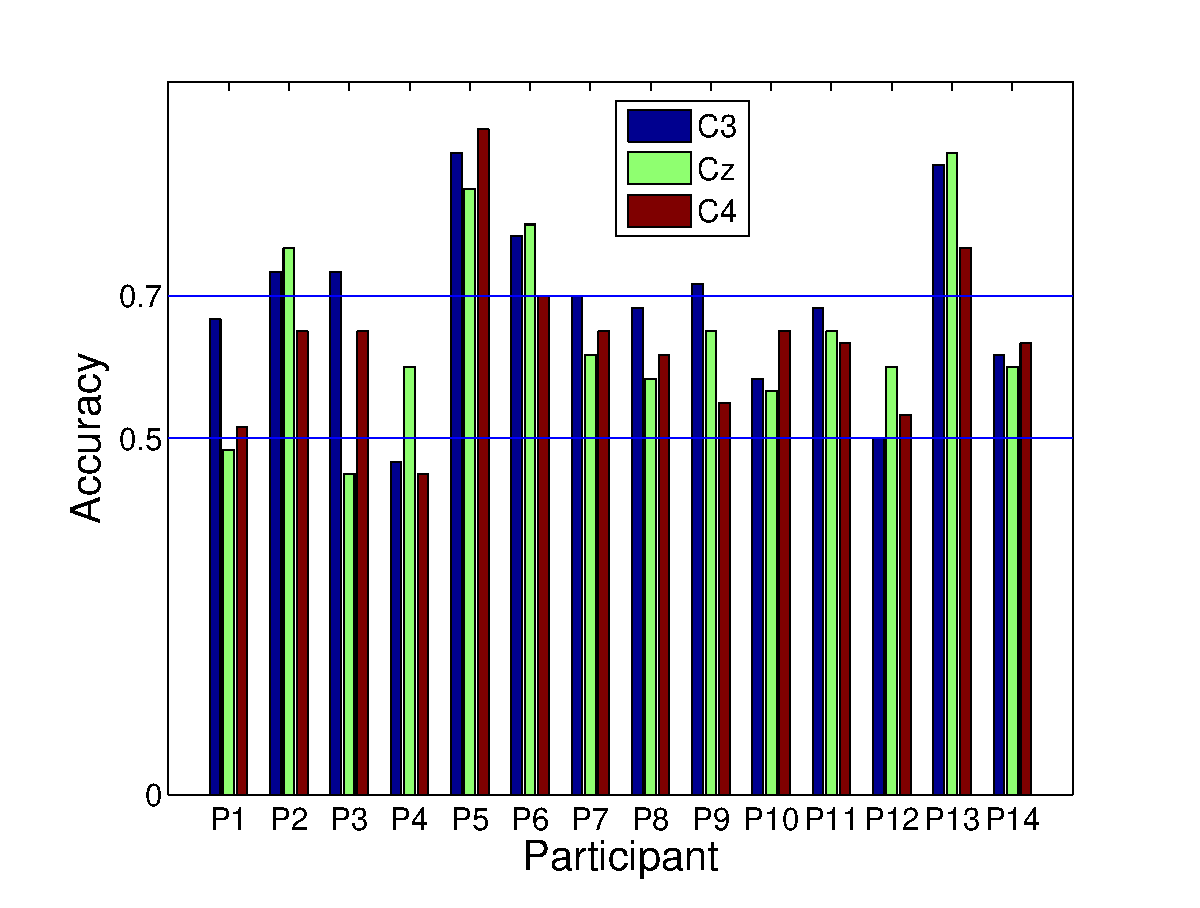
\includegraphics[scale=0.45]{images/DatasetMIBCISimulation1}}
      \caption{\centering Accuracy for the BCI Simulation classifying Baseline vs. RH (Right Hand) motor imagery.}
      \label{figure3}
   \end{figure} 	
	\end{frame}	  
	
	
	\begin{frame}
	\frametitle{$\mu$ Rhythm}
   \begin{figure}[thpb]
      \centering
      \setlength\fboxsep{0pt}
	  \setlength\fboxrule{0.5pt}
       \fbox{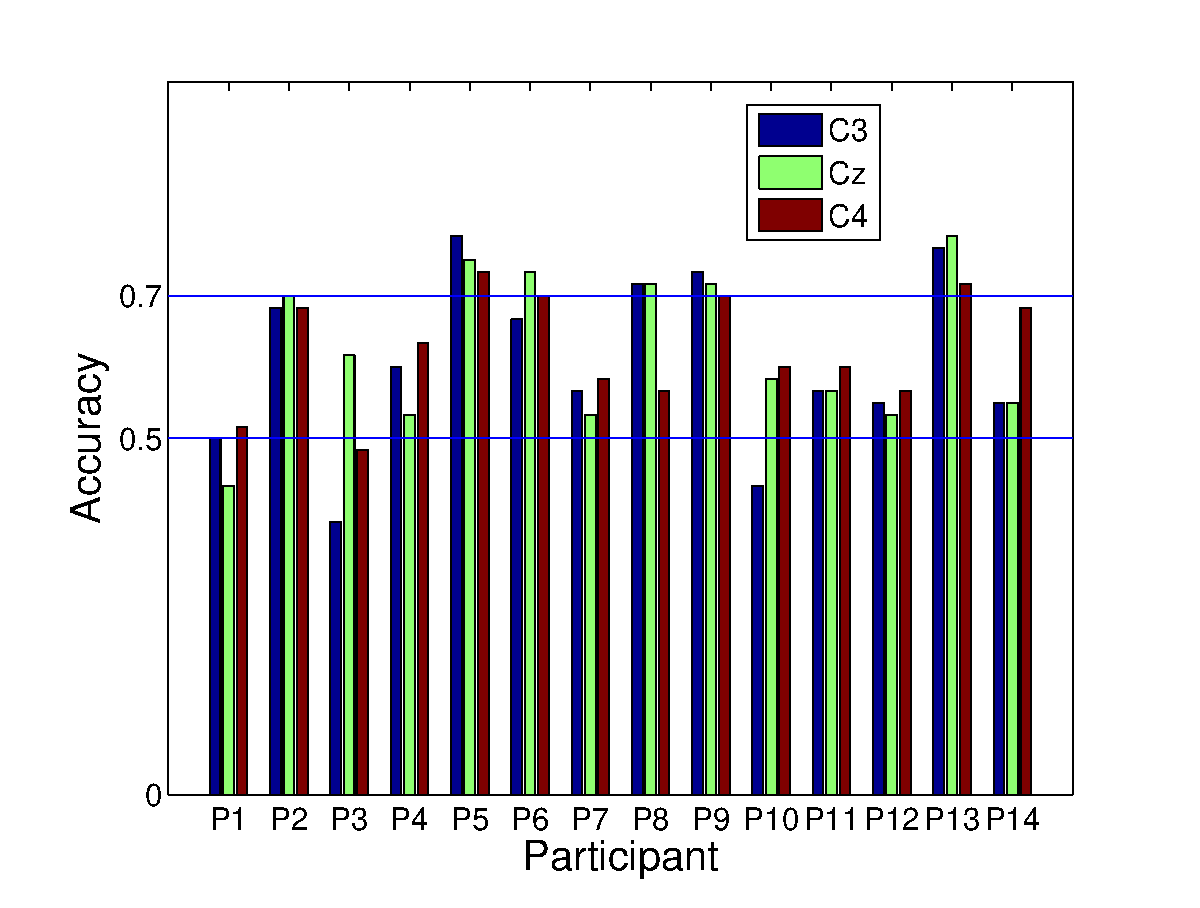
\includegraphics[scale=0.45]{images/DatasetMIBCISimulation2}}
      \caption{\centering Accuracy for the BCI Simulation classifying Baseline vs. FM (Feet Movement) motor imagery.}
      \label{figure3}
   \end{figure} 	
	\end{frame}	  
	    
\begin{frame}
\frametitle{Experimental Validation}
\begin{center}
\LARGE The P300 Waveform
\end{center}
\end{frame}

\begin{frame}
\frametitle{P300-Based Speller Matrix}
\begin{figure}[h!]
\centering
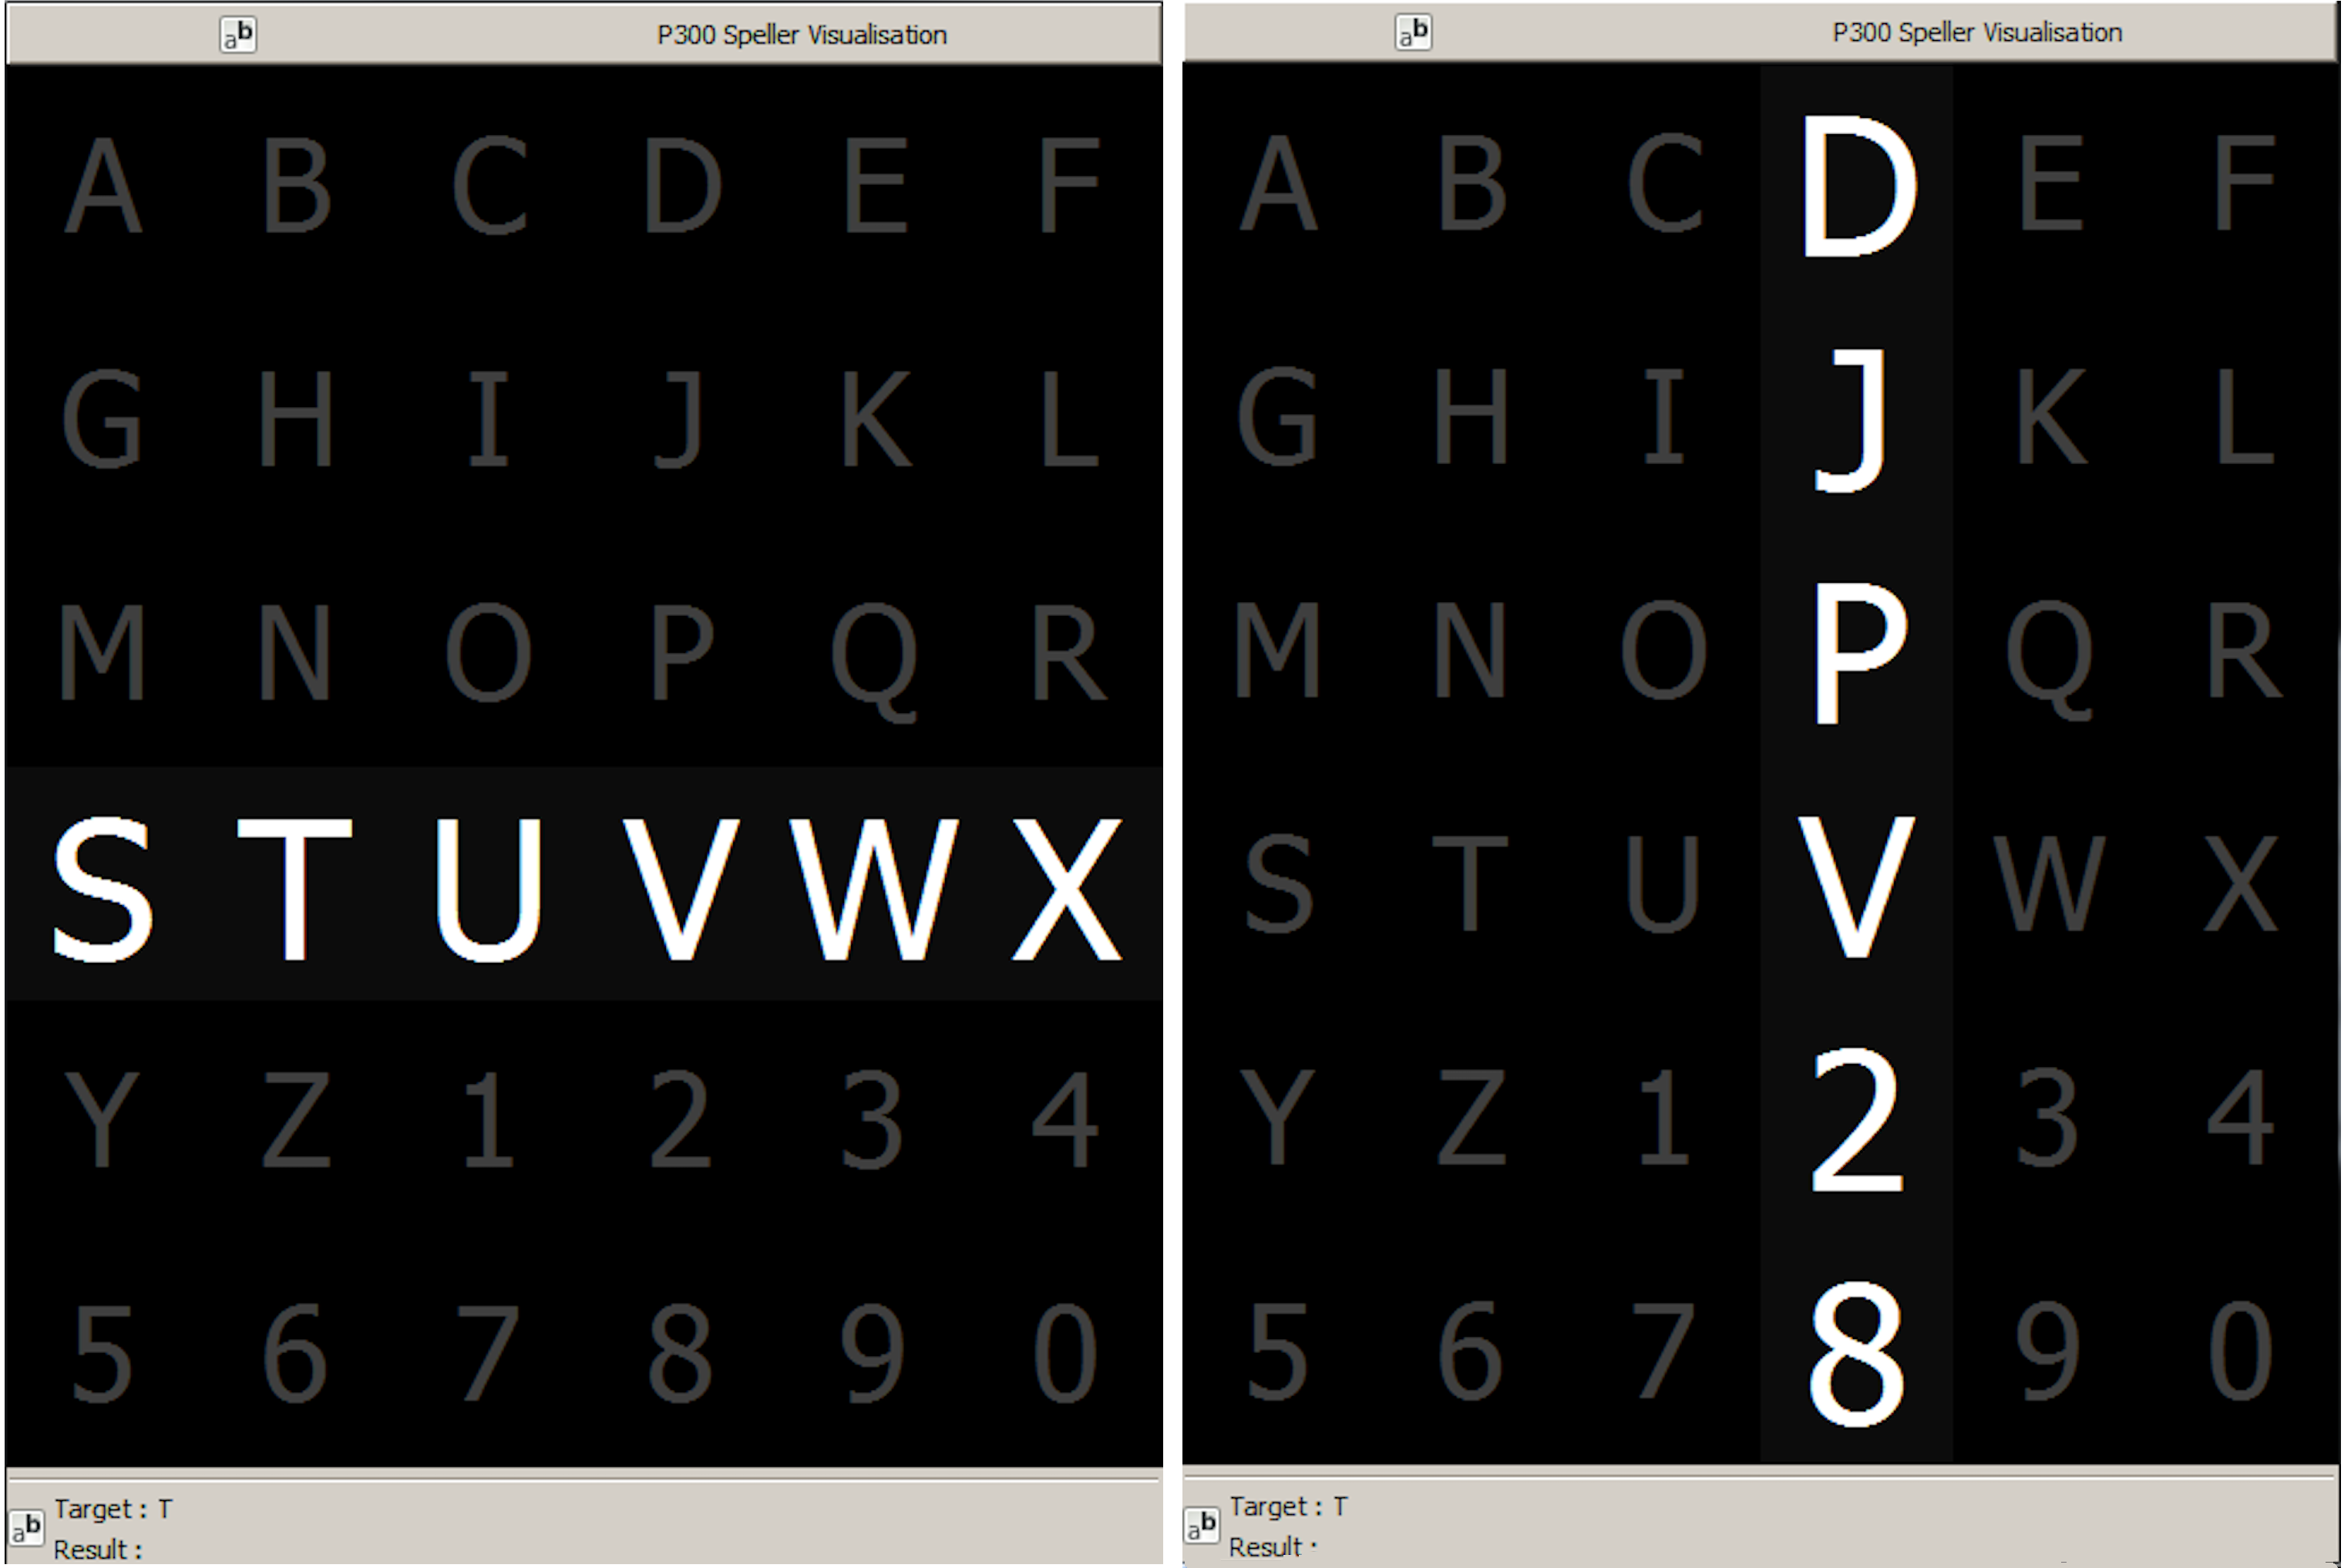
\includegraphics[width=12.5cm,height=6.7cm]{images/openvibep300matrix.png}
\caption{OpenVibe software $6 \times 6$ Speller Matrix.  Rows and columns flash in random permutations.}
\label{fig:p300matrix}
\end{figure}
\end{frame}    


\begin{frame}
\frametitle{The P300 Waveform - Signal Preprocessing}
\begin{figure}[h!]
\centering
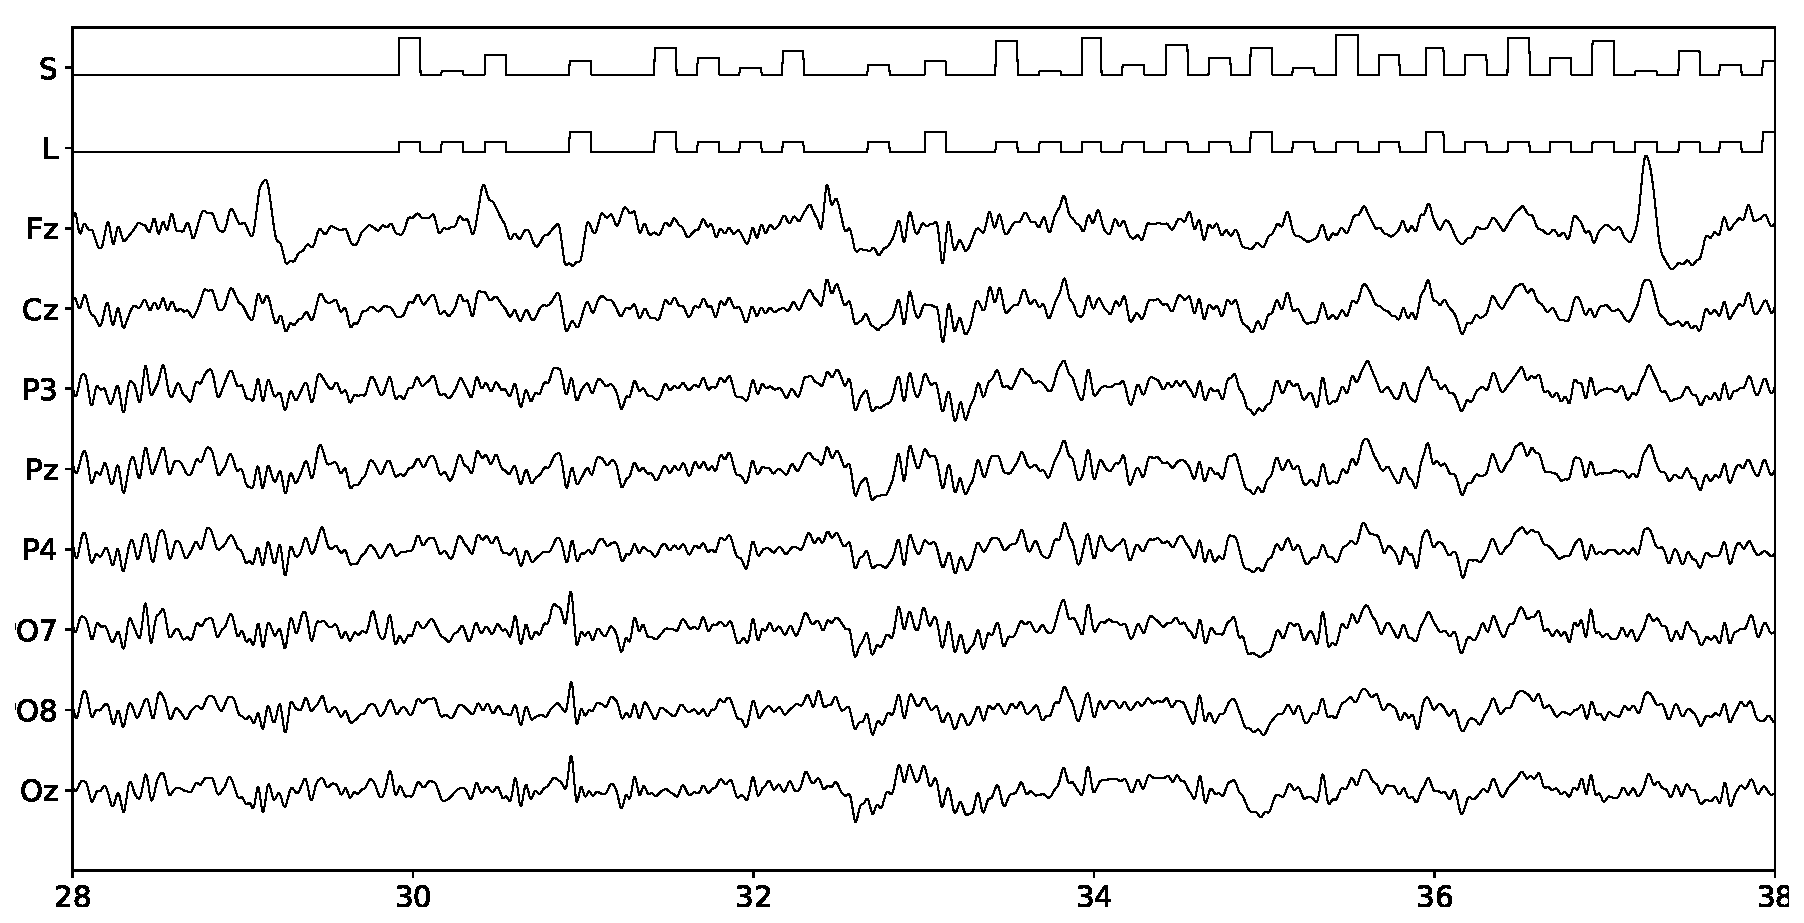
\includegraphics[width=.45\linewidth]{images/nogain.eps}
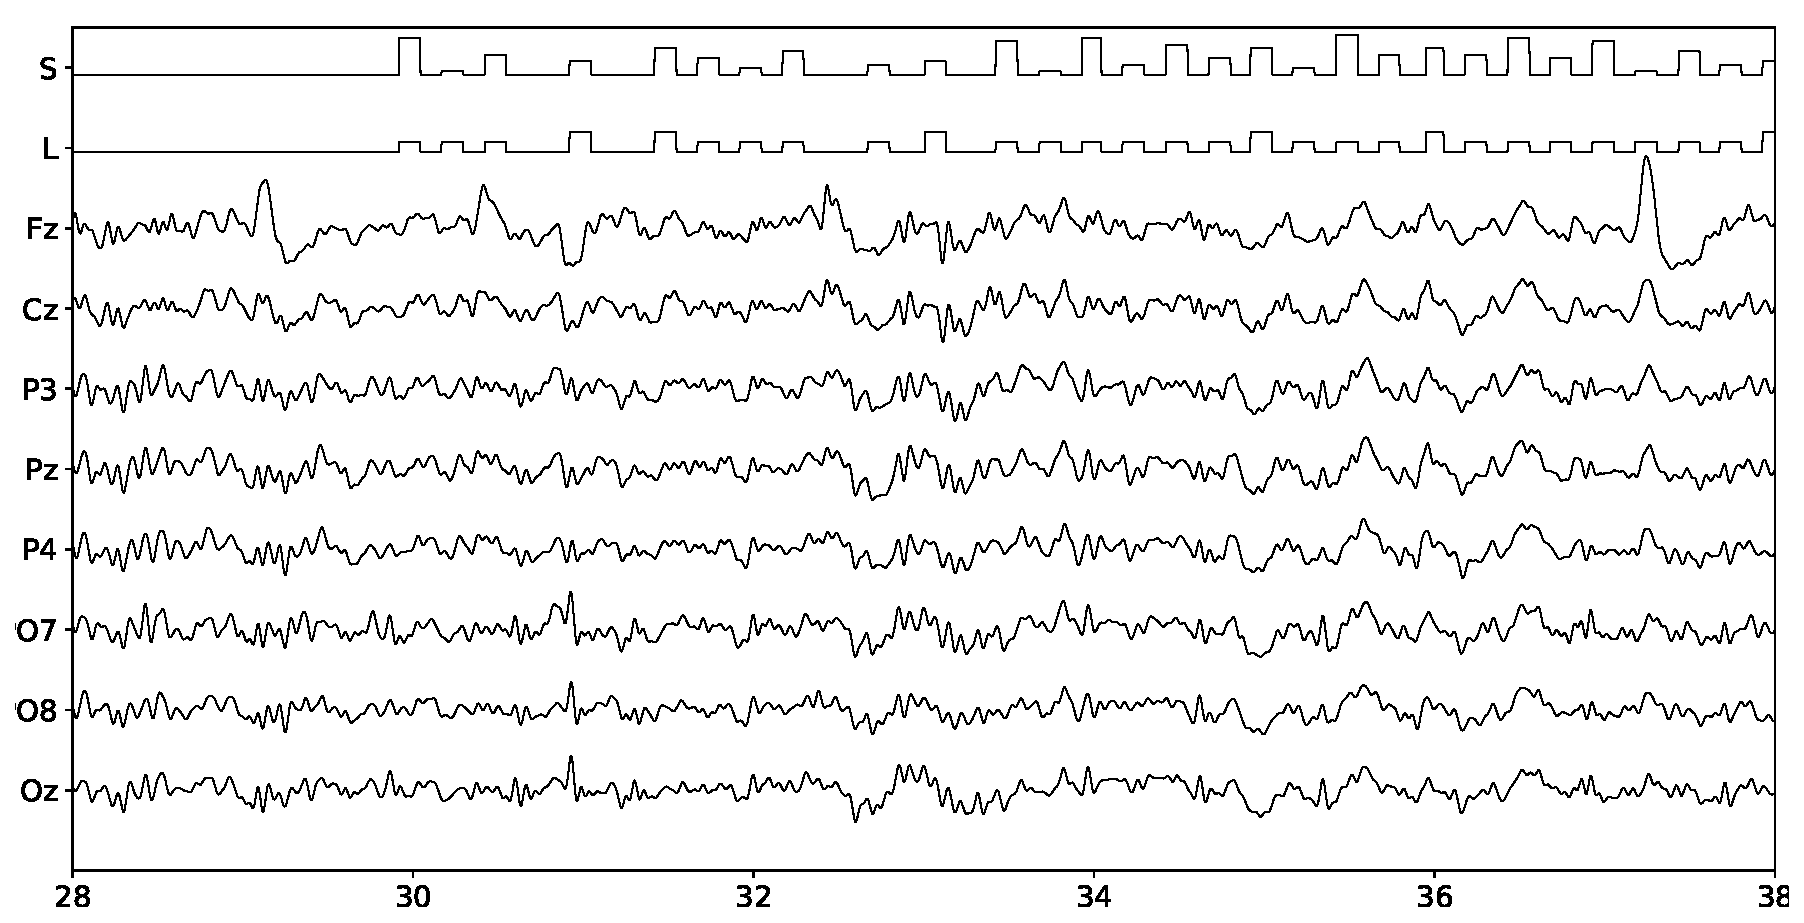
\includegraphics[width=.45\linewidth]{images/singlegain.eps}\\
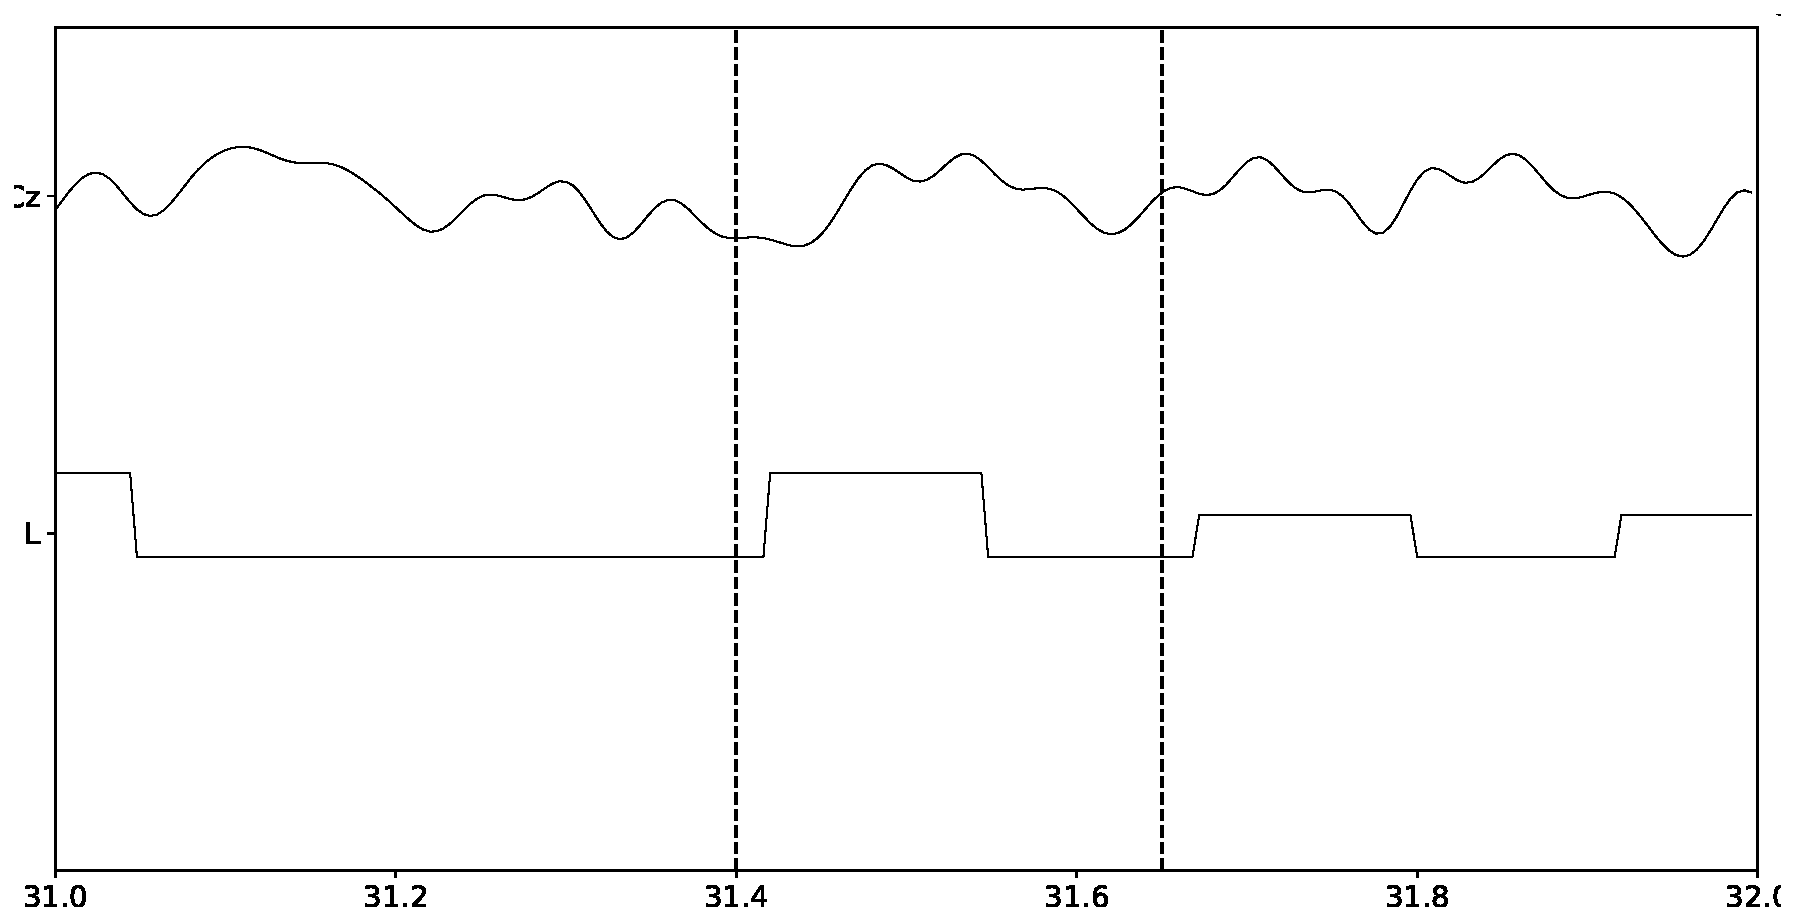
\includegraphics[width=.45\linewidth]{images/nogainzoomhit.eps}
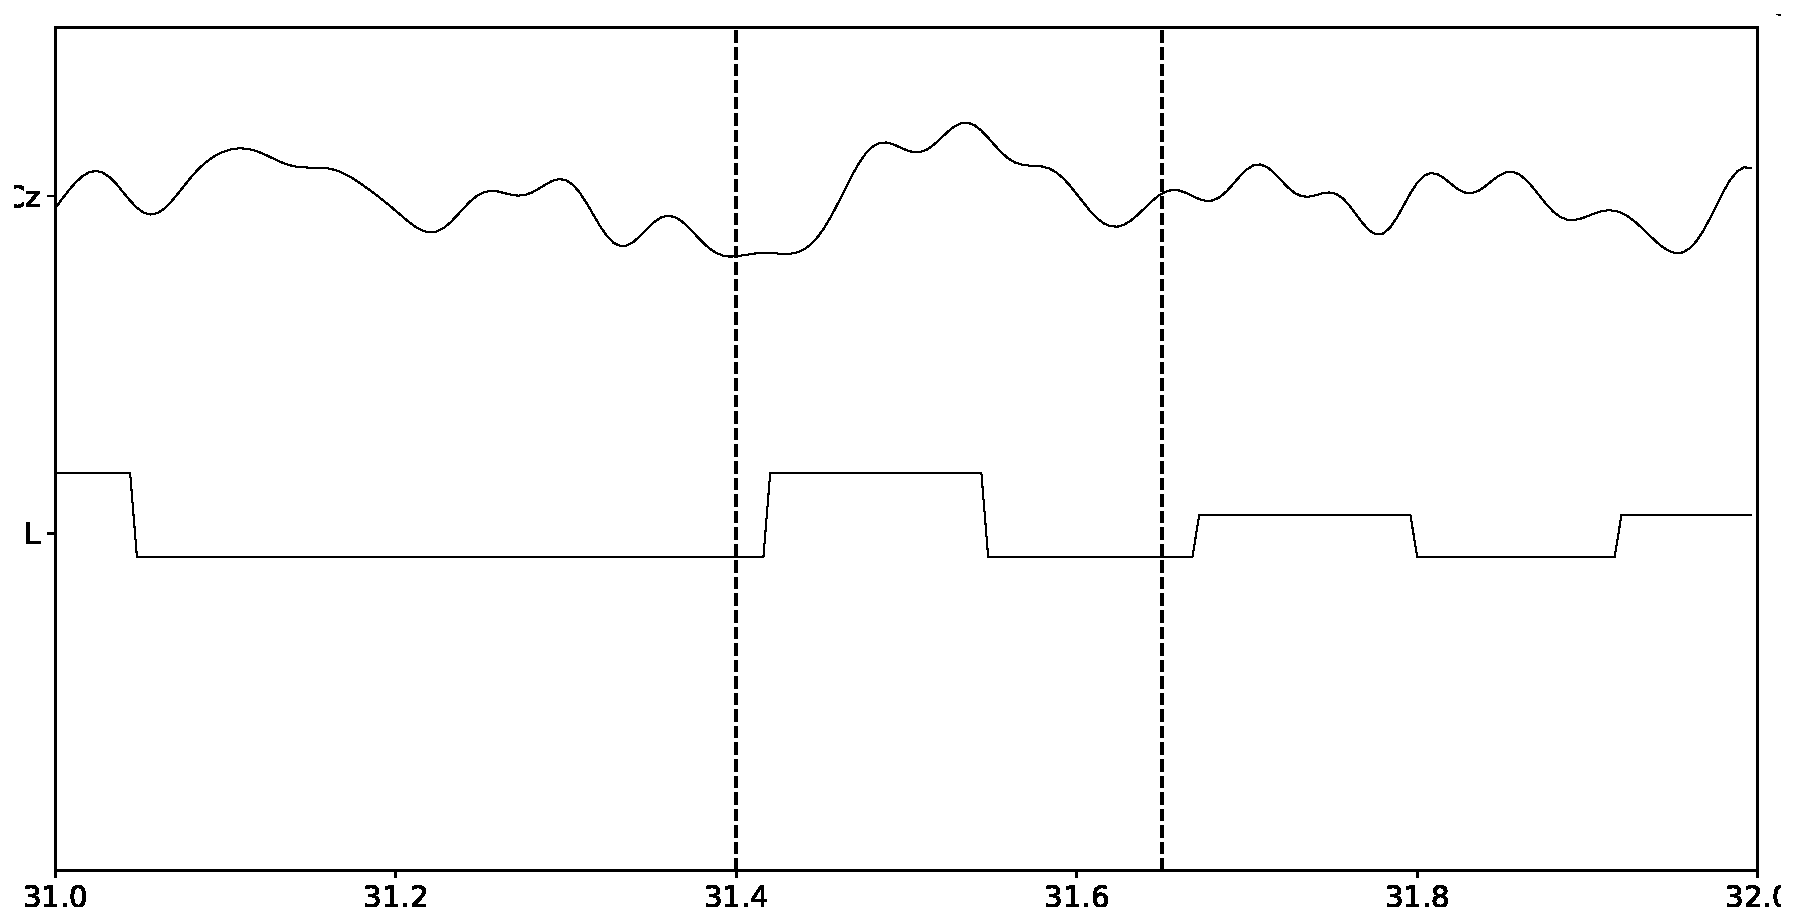
\includegraphics[width=.45\linewidth]{images/singlegainzoomhit.eps}
\label{fig:gains}
\end{figure}
\end{frame}



\begin{frame}
\frametitle{Signal Averaging}
\begin{center}
\begin{figure}[htb]
\centering
\includegraphics[scale=0.5]{images/classificationgraph.pdf}
\label{fig:classification}
\end{figure}
\end{center}
\end{frame}     


\begin{frame}
\frametitle{P300-Based BCI Speller - Letter Identification}
\begin{center}
\vspace{-\baselineskip}
\begin{equation}
\hat{row} = \arg \min_{l \in \{1,\dots,6\}} \sum_{h=1}^{\gls{k}}  {\left\lVert \mathbf{q}^{(l,bpc)} -  \mathbf{d}_{h}^{(bpc)} \right\rVert}  ^{2}
\label{eq:multiclassificationrow}
\end{equation}
\begin{equation}
\hat{col} = \arg \min_{l \in \{7,\dots,12\}} \sum_{h=1}^{\gls{k}}  {\left\lVert \mathbf{q}^{(l,bpc)} -  \mathbf{d}_{h}^{(bpc)} \right\rVert}  ^{2}
\label{eq:multiclassificationcol}
\end{equation}

\begin{itemize}
\item $l \in \{1,\dots,12\}$ speller matrix row/col index.
\item $\hat{row}$  and $\hat{col}$ predicted row and col of the speller matrix.
\item $\mathbf{q}^{(l,bpc)} $ query descriptor of matrix index $l$.
\item $\mathbf{d}_{h}^{(bpc)} $ neighbors descriptors from the template.
\item $\mathbf{d}_{h}^{(bpc)} \in N_T(  \mathbf{q}^{(l,bpc)} )$.
\item $\gls{k}$ the number of neighbors to pick from the template~\footfullcite{Boiman2008}.
\end{itemize}

\end{center}
\end{frame}   


\begin{frame}
\frametitle{P300 Datasets}
\begin{center}
\begin{itemize}
 \item<1-> \Fontre Dataset I - P300 ALS Public Dataset 
 \begin{itemize}
 \item 8 subjects, 8 channels, Fs=256 Hz, 7 words, 5 letters, ISI=0.125 s, 10 epochs
 \end{itemize}
 \item<2-> \Fontre Dataset II - P300 for Healthy subjects
 \item<3-> \Fontre Dataset III - P300 Pseudo-Real Dataset 
 \begin{itemize}
 \item 1 subject, null-signals
 \end{itemize}
 \item<4-> \Fontre Dataset IV - P300 Dataset IIb BCI Competition II (2003) 
 \begin{itemize}
 \item 1 subject, 64 channels, Fs=240 Hz, 73 trials, 42 train and 31 test, ISI=0.25 s, 15 epochs
 \end{itemize}
\end{itemize}
\end{center}
\end{frame} 

\begin{frame}
\frametitle{Alternative Methods used for comparison}
\begin{center}
\begin{itemize}
 \item<1-> \Fontre Support Vector Machine SVM
 \item<2-> \Fontre Stepwise Linear Discriminant Analysis SWLDA.
 \item<3-> \Fontre Permutation Entropy %(m=3, w=10)
 \item<4-> \Fontre Matching Pursuit 1 MP-1 %(Daubechies least-symmetric wavelets, 2 vanishing moments)
 \item<5-> \Fontre Matching Pursuit 2 MP-2
 \item<6-> \Fontre Slope Horizontal Chain Code SHCC.
\end{itemize}
\end{center}
\end{frame} 


\begin{frame}
\frametitle{P300 Waveform - Dataset I}
\begin{center}
\begin{table}[h!]
\caption{Character recognition rates public dataset of ALS patients.}
\centering
%% \tablesize{} %% You can specify the fontsize here, e.g.  \tablesize{\footnotesize}. If commented out \small will be used.
\begin{tabular}{c|cc|cc}
\toprule
\textbf{Participant}	&  $bpc$ 	&  HIST &  $bpc$	&  Single Channel SVM \\
\midrule
1     &     Cz   &   $35\%$    &  Cz   & $15\%$   \\
2     &     Fz   &   $85\%$      &  PO8   & $25\%$   \\
3     &     Cz   &   $25\%$    &  Fz   & $5\%$   \\
4     &     PO8 &   $55\%$   &  Oz   & $5\%$    \\
5     &     PO7 &   $40\%$    &  P3   & $25\%$   \\
6     &     PO7 &   $60\%$  &  PO8   & $20\%$    \\
7     &     PO8 &   $80\%$   &  Fz   & $30\%$     \\
8     &     PO7 &   $95\%$     &  PO7   & $85\%$ \\

%\bottomrule
\end{tabular}
\label{tab:resultsals}
\end{table}
\end{center}
\end{frame} 


\begin{frame}
\frametitle{Character Identification Rates - Dataset I}
\begin{center}
\begin{figure}[h!]
\centering
\includegraphics[width=9.5cm]{images/performance.eps}
\label{fig:performance}
\end{figure}
\end{center}
\end{frame} 


\begin{frame}
\frametitle{The P300 Waveform - Dataset II}
\begin{center}
\begin{table}[h!]
\caption{Character recognition rates for the Dataset of Healthy volunteers.}
\centering
%% \tablesize{} %% You can specify the fontsize here, e.g.  \tablesize{\footnotesize}. If commented out \small will be used.
\begin{tabular}{c|cc|cc}
\toprule
\textbf{Participant}	&  $bpc$	&  HIST &  $bpc$	&  Single Channel SVM \\
\midrule
1     &     Oz   &   $40\%$  &  Cz   &  $10\%$    \\
2     &     PO7   &   $30\%$      &  Cz   & $5\%$   \\
3     &     P4   &   $40\%$    &  P3   & $10\%$    \\
4     &     P4 &   $45\%$    &  P4   & $35\%$     \\
5     &     P4 &   $60\%$  &  P3   & $10\%$     \\
6     &     Pz &   $50\%$ &  P4   & $25\%$     \\
7     &     PO7 &   $70\%$  &  P3   & $30\%$     \\
8     &     P4 &   $50\%$    &  PO7   & $10\%$    \\

%\bottomrule
\end{tabular}
\label{tab:resultsown}
\end{table}
\end{center}
\end{frame} 


\begin{frame}
\frametitle{Dataset I Multichannel comparison}
\begin{center}
\begin{table}[h!]
\centering
%% \tablesize{} %% You can specify the fontsize here, e.g.  \tablesize{\footnotesize}. If commented out \small will be used.
\begin{tabular}{c|cc|c|c}
\toprule
%\textbf{Participant}	&  \textbf{BPC}	& \multicolumn{2}{c}{Character Recognition Rates}\\
%\cline{1-5} \\
\textbf{Participant}	&  $bpc$	&  HIST & Multichannel SWLDA & Multichannel SVM \\
                                    &  for HIST        &           &                                       &   \\
\midrule
1     &     Cz   &   $35\%$  & $45\%$  & $40\%$\\
2     &     Fz   &   $85\%$  & $30\%$   & $50\%$   \\
3     &     Cz   &   $25\%$  & $65\%$ & $55\%$   \\
4     &     PO8 &   $55\%$ & $40\%$  & $50\%$   \\
5     &     PO7 &   $40\%$ & $35\%$  & $45\%$   \\
6     &     PO7 &   $60\%$ &  $35\%$  & $70\%$   \\
7     &     PO8 &   $80\%$ & $60\%$   & $35\%$   \\
8     &     PO7 &   $95\%$  & $90\%$   & $95\%$  \\

%\bottomrule
\end{tabular}
\label{tab:resultsalsswlda}
\end{table}
\end{center}
\end{frame} 


\begin{frame}
\frametitle{Dataset II Multichannel Comparison}
\begin{center}
\begin{table}[h!]
\centering
%% \tablesize{} %% You can specify the fontsize here, e.g.  \tablesize{\footnotesize}. If commented out \small will be used.
\begin{tabular}{c|cc|c|c}
\toprule
%\textbf{Participant}	&  \textbf{BPC}	& \multicolumn{2}{c}{Character Recognition Rates}\\
%\cline{1-5} \\
\textbf{Participant}	&  $bpc$ 	&  HIST & Multichannel SWLDA & Multichannel SVM  \\
                                    &  for HIST        &           &                                       &   \\
\midrule
1     &     Oz   &     $40\%$  &     $65\%$  &     $40\%$ \\
2     &     PO7   &     $30\%$ &   $15\%$  &     $10\%$ \\
3     &     P4   &     $40\%$ &     $50\%$  &     $25\%$ \\
4     &     P4   &     $45\%$ &     $40\%$  &     $20\%$ \\
5     &     P4   &      $60\%$ &    $30\%$  &     $20\%$ \\
6     &     Pz   &      $50\%$ &    $35\%$  &     $30\%$ \\
7     &     PO7   &      $70\%$ &  $25\%$  &     $30\%$ \\
8     &     P4   &      $50\%$ &    $35\%$  &     $20\%$ \\
%\bottomrule
\end{tabular}
\label{tab:resultsownswlda}
\end{table}
\end{center}
\end{frame} 

\begin{frame}
\frametitle{Character Identification Rates for Dataset I and II}
\begin{center}
\begin{figure}[h!]
\centering
\includegraphics[width=10cm]{images/boxplots.png}
\caption{Quade test with $p=0.55$.}
\label{fig:boxplots}
\end{figure}
\end{center}
\end{frame} 

\begin{frame}
\frametitle{P300 Waveforms for Subject 8 (A) and 3 (B)}
\begin{center}
\begin{figure}[h!]
\centering
\includegraphics[height=7cm,width=1\textwidth]{images/subject.png}\label{subject8}
\label{fig:p300templates}
\end{figure}
\end{center}
\end{frame} 
    

\begin{frame}
\frametitle{P300 Pseudo-Real Dataset III Performance Results }    
\begin{table}[h!]
\centering
%% \tablesize{} %% You can specify the fontsize here, e.g.  \tablesize{\footnotesize}. If commented out \small will be used.
\begin{tabular}{ccccc}
\toprule
\textbf{Method}	& \textbf{$\gls{bpc}$} &   \multicolumn{3}{c}{Performance} \\
%\cline{3-5} \\
 	&  &  \textbf{Experiment 1} & \textbf{Experiment 2}	& \textbf{Experiment 3}\\
\midrule
MP 1 & PO8  & $67\%$ & $15\%$ & $50\%$\\
MP 2 & PO7 & $24\%$ & $6\%$ & $10\%$\\
HIST  & PO8 & $91\%$ & $18\%$ & $66\%$\\
PE     & Cz & $61\%$ & $9\%$ & $32\%$\\
SHCC & P4 & $98\%$ & $31\%$ & $80\%$\\
SVM     & PO8  & $78\%$ & $7\%$ & $53\%$\\
\bottomrule
\end{tabular}
\label{tab:results}
\end{table}    
\end{frame} 

\begin{frame}
\frametitle{The P300 Wave - Dataset IV BCI Competition 2003 }    
\begin{table}[h!]
\centering
%% \tablesize{} %% You can specify the fontsize here, e.g.  \tablesize{\footnotesize}. If commented out \small will be used.
\begin{tabular}{ccc}
\toprule
\textbf{Method}	& \textbf{$\gls{bpc}$} &  \textbf{Performance} \\
\midrule
MP 1 & FC2  & $50\%$ \\
MP 2 & CPz & $22\%$ \\
HIST  & Cz & $67\%$ \\
PE     & PO8 & $22\%$ \\
SHCC & Cz & $61\%$ \\
SVM     & C1  & $32\%$ \\
\bottomrule
\end{tabular}
\label{tab:bcicompetitionresults}
\end{table}
\end{frame} 
    
    \section{Conclusion}
\begin{frame}
\frametitle{Conclusion}
\begin{center}
\LARGE Conclusion
\end{center}
\end{frame}

\begin{frame}
\frametitle{Findings}
\begin{center}
\begin{itemize}
\item \Fontre $\alpha$ and $\mu$ waves can be identified by their waveforms.
\item \Fontre Occipital regions more prominent P300 waveforms.
\item \Fontre The stability of ERP transient components in ALS patients. 
\begin{itemize}
\item Mann-Whitney U Test, $p=0.46$
\end{itemize}
\item \Fontre Latency jitter. 
\begin{itemize}
\item Wilcoxon rank sum test, one tail, $p=0.0022$
\end{itemize}
\item \Fontre Component Amplitude resistance. 
\begin{itemize}
\item Wilcoxon rank sum test, two tails, $p=0.17$
\end{itemize}
\end{itemize}
\end{center}
\end{frame}

\begin{frame}
\frametitle{Thesis Contributions}
\begin{center}
\begin{itemize}
\item \Fontre Method to construct analyzable image plots.
\item \Fontre EEG Waveform Feature Extraction Procedure.
\item \Fontre SIFT extension and modification: HIST.
\item \Fontre Classification algorithm.
\end{itemize}
\end{center}
\end{frame}        

\begin{frame}
\frametitle{Practical Contributions}
\begin{center}
\begin{itemize}
\item \Fontre P300-Dataset on Kaggle.
\item \Fontre EEGWave - Code Ocean Reproducible Research Platform.
\item \Fontre Online Speller Application based on OpenVibe and LSL.
\item \Fontre BCI Online Blog.
\item \Fontre Matlab toolbox for Computer Vision-EEG Analysis.
\end{itemize}
\end{center}
\end{frame} 
    
\begin{frame}
\frametitle{Conclusion}
\begin{center}
\begin{itemize}
\item \Fontre EEG Waveforms can be objectively analyzed.
\item \Fontre Inherent Intelligible System may foster clinical collaboration.
\end{itemize}
\end{center}
\end{frame}    
    
%\begin{frame}
%\frametitle{Conclusion}
%\begin{center}
%\LARGE Dissertation Contributions
%\end{center}
%\end{frame}
%


    \begin{frame}
        \frametitle{Future Work}
        \begin{center}
            \begin{itemize}
                \item \Fontre BCI Paradigms Potential Universal Applicability
                \item \Fontre Multichannel extension.
                \item \Fontre Keypoint localization.
                \item \Fontre Neuroimaging.
            \end{itemize}
        \end{center}
    \end{frame}       
   
        \section{Questions}
    \begin{frame} %Biblio
        \frametitle{Questions}
        \begin{center}
        \LARGE Questions?
        \end{center}
    \end{frame}
    
    \begin{frame} %Biblio
        \begin{center}
        \LARGE Thank you very much
        \end{center}
    \end{frame}


\begin{frame}
\frametitle{Preprocessing steps}
\begin{itemize}
\item Notch filter:
\item Band-pass filter
\item Decimation or Downsizing:
\item Segmentation
\item Baseline Removal
\item Artifact Rejection
\item Spatial Filter
\end{itemize}
An excellent review can be found here~\footfullcite{Simons2016}.
\end{frame}



\begin{frame}
\frametitle{Histogram of Gradient Orientation - Trilinear Interpolation}
\begin{equation}
 \omega_{ij}(\mathbf{v}) = \omega \bigg ( \frac{5 \;v_x}{\gls{Deltas} \; \gls{St}} - x_i \bigg ) \omega \bigg ( \frac{5 \; v_y}{\gls{Deltas} \; \gls{Sv}} - y_i \bigg ) 
\label{eq:ij}
\end{equation}

\begin{equation}
 \omega_\mathrm{ang}(\alpha) = \sum_{r=-1}^{1} \omega \bigg ( \frac{8\alpha}{2\pi} + 8r \bigg )
\label{eq:wang}
\end{equation}
\end{frame}

%\begin{frame}
%\frametitle{Sample frame title}
% 
%In this slide, some important text will be
%\alert{highlighted} beause it's important.
%Please, don't abuse it.
 
%\begin{block}{Remark}
%Sample text
%\end{block}
% 
%\begin{alertblock}{Important theorem}
%Sample text in red box
%\end{alertblock}
% 
%\begin{examples}
%Sample text in green box. "Examples" is fixed as block title.
%\end{examples}
%\end{frame}
	
	\begin{frame}
	\frametitle{EEG Signal Plot - Zero Level and Standardization}
	\begin{center}

\begin{equation}
\tilde{x}(n,c) =  \frac{ x(n,c) - \bar{x}(c) }{ \hat{\sigma}(c) } 
\label{eq:standarizedaverages}
\end{equation}

\begin{equation}
z(c) = \left \lfloor{ \frac{\max_{n} \tilde{x}(n,c)  - \min_{n} \tilde{x}(n,c) }{2} }\right \rfloor -   \left \lfloor{ \frac{\max_{n} \tilde{x}(n,c)  + \min_{n} \tilde{x}(n,c)}{ 2} }\right \rfloor
\label{eq:zerolevel}
\end{equation}

	\end{center}
	\end{frame}

	\begin{frame}
	\frametitle{EEG Signal Plot}
	\begin{center}
	
\begin{equation}
\mathcal{I}^{(c)}(z_1,z_2) = \left\{ \begin{array}{rl}
255 & \text{if} \   z_1 = \gamma_{t} \  n \quad \text{and}  \quad z_2 = \left\lfloor \gamma \; \tilde{x}(n,c) \right\rceil + z(c) \\
0   & \mbox{otherwise}
\end{array}\right.
\label{eq:images}
\end{equation}

		\includegraphics[scale=2]{images/SignalSample.png} 
		\includegraphics[scale=2]{images/SignalSample2.png} 
		
% \eqno{(2)}

        \end{center}
    \end{frame}


%    \begin{frame}
  %      \frametitle{Signal Transformation}
 %       \begin{center}           
   %     \includegraphics[scale=4]{images/SignalTransformation.png} 
     %   \end{center}
    %\end{frame}
    
    
    \begin{frame}
        \frametitle{SIFT Descriptors}
        \begin{center}
   			\begin{figure}[thpb]
      			\centering
      			\setlength\fboxsep{0pt}
	  			\setlength\fboxrule{0.5pt}
       			\fbox{\includegraphics[scale=0.7]{images/BaselineDescriptor.png}}
      			\caption{\centering SIFT Descriptor $ [ z_1, z_2, \theta, \sigma ] $ where $ (z_1, z_2) $ are the 2D coordinates where the \textit{Keypoint} is located, $ \theta $ is the descriptor general orientation and $ \sigma $ is the descriptor size. }
      			\label{figure1}
   			\end{figure}        
        \end{center}
    \end{frame}   
    

    
    \begin{frame}
        \frametitle{SIFT Descriptors}
        \begin{center}
   			\begin{figure}[thpb]
      		\centering
      		\setlength\fboxsep{0pt}
	  		\setlength\fboxrule{0.5pt}
       		\fbox{\includegraphics[scale=0.6]{images/EasyDescriptorSample1.png}}
       		\fbox{\includegraphics[scale=0.6]{images/EasyDescriptorSample2.png}}
      		\caption{\centering Sample Descriptors from artificial signals.}
      		\label{figure1}
   			\end{figure}        
        \end{center}
    \end{frame}       
        
    \begin{frame}
        \frametitle{SIFT Descriptors}
        \begin{center}
   			\begin{figure}[thpb]
      		\centering
      		\setlength\fboxsep{0pt}
	  		\setlength\fboxrule{0.5pt}
       		\fbox{\includegraphics[scale=0.48]{images/BaselineDescriptorValues2.png}}
      		\caption{\centering Sample descriptor values of the given patch.}
      		\label{figure1}
   			\end{figure}        
        \end{center}
    \end{frame}   
    
    %\begin{frame}
     %   \frametitle{SIFT Descriptors}
       % \begin{center}
   		%	\begin{figure}[thpb]
      	%		\centering
      	%		\setlength\fboxsep{0pt}
	  	%		\setlength\fboxrule{0.5pt}
       	%		\fbox{\includegraphics[scale=0.4]{images/BaselineDescriptorRepresentation.png}}
      	%		\caption{\centering Descriptor values and their representation as intensity gradients.}
      	%		\label{figure1}
   		%	\end{figure}        
       % \end{center}
    %\end{frame}   
    

\begin{frame}
\frametitle{Brain Computer Interfaces - Chronology}
\begin{center}

\begin{chronology}[5]{1966}{2014}{90ex}[\textwidth]
\event{1966}{Kamiya, Neurofeedback for $\alpha$ waves}
\event{1969}{Fetz, Operand Conditioning}
\event{1973}{Vidal, first use of BCI word}
\event{1987}{Donchin \textbf{P300}}
\event{1989}{Hiraiwa, Bereitschaftspotentials}
\event{1991}{Wolpaw $\mu$ \textbf{Wadsworth BCI}}
\event{1993}{Pfurtscheller SMR \textbf{Graz BCI}}
\event{1995}{Jane Huggins invasive BrainGate}
\event{1997}{Anderson, Mental Tasks}
\event{1999}{Birmahuer SCP}
\event{2001}{Nicolelis, invasive BCI on primates}
\event{2003}{Middendorf, SSVEP}
\event{2006}{Millan, ErrP}
\event{2008}{Blankertz, adaptive \textbf{Berlin BCI}}
\event{2010}{Schalk, ECoG BCI}
\event{2012}{Zander, Passive BCI \textbf{pBCI}}
%\event{\decimaldate{25}{12}{2001}}{three}
\label{fig:story}
\end{chronology}
\end{center}
\end{frame}     
    


        
   %\begin{frame}     
   %\begin{figure}[thpb]
    %  \centering
    %  \setlength\fboxsep{0pt}
	 % \setlength\fboxrule{0.5pt}
     %  \fbox{\includegraphics[scale=0.3]{images/DatasetPhysionetAccuracyPerChannel}}
     %  \fbox{\includegraphics[scale=0.3]{images/DatasetPhysionetBoxPlots}}
     % \caption{10-KFold CrossValidation}
     % \label{figure2}
   %\end{figure}  
    %\end{frame}
    


	
	

    

    
\begin{frame}    
\begin{figure}[htb]
\centering
\includegraphics[scale=0.4]{images/neuralplanes.png}
\includegraphics[scale=0.4]{images/neuroanatomy.png}
\caption[Neuroanatomical structures of the brain]{Neuronal Planes regularly used in neuroscience research.  In BCI they are used to understand electrode location and spatial filters.}
\label{fig:neuroanatomy}
\end{figure}
\end{frame}

\begin{frame}    
\begin{figure}[]
\centering
\includegraphics[height=4cm,width=1\textwidth]{images/volconduction1.png}\\
\includegraphics[height=4cm,width=1\textwidth]{images/volconduction2.png}
\caption[EEG Volume Conduction]{A source signal with positive/negative polarity is generated in a very specific region of the brain but due to volume conduction their influence affects a widespread area of the scalp where sensors are located (Image of the brain from Swartz Center for Computational Neuroscience).}
\label{fig:volconduction}
\end{figure}
\end{frame}

\begin{frame}   
\begin{figure}[]
\centering
\includegraphics[height=4cm,width=7cm]{images/emotivsubject.jpg}
\includegraphics[height=4cm,width=7cm]{images/gTecsubject.jpg}
\caption[Wearable portable Digital Electroencephalograph]{Digital and wearable electroencephalographs.}
\label{fig:digitalelectroencephalograph}
\end{figure}
\end{frame}


\begin{frame}   
\begin{figure}[]
\centering
\includegraphics[height=7.8cm,width=1\textwidth]{images/hype.png}
\caption[Wearable portable Digital Electroencephalograph]{Digital and wearable electroencephalographs.}
\label{fig:digitalelectroencephalograph}
\end{figure}
\end{frame}

\begin{frame}   
\begin{figure}[]
\centering
\includegraphics[height=7.8cm,width=1\textwidth]{images/Cic.png}
\caption[Wearable portable Digital Electroencephalograph]{Digital and wearable electroencephalographs.}
\label{fig:digitalelectroencephalograph}
\end{figure}
\end{frame}  

\begin{frame}   
\begin{figure}[]
\centering
\includegraphics[height=9cm,width=1\textwidth]{images/Convocatoria.png}
\caption[Wearable portable Digital Electroencephalograph]{Digital and wearable electroencephalographs.}
\label{fig:digitalelectroencephalograph}
\end{figure}
\end{frame}  

\begin{frame}   
\begin{figure}[]
\centering
\includegraphics[height=9cm,width=1\textwidth]{images/Papers.png}
\caption[Wearable portable Digital Electroencephalograph]{Digital and wearable electroencephalographs.}
\label{fig:digitalelectroencephalograph}
\end{figure}
\end{frame}  

\begin{frame}
\frametitle{The P300 Wave}
\begin{center}
Additionally, the stability of the P300 component waveform has been extensively studied in patients with ALS ~\footfullcite{SellersandEmanuelDonchin2006,TomohiroMadarame2008,Nijboer2009,Mak2012,McCane2015} where it was found that these patients have a stable P300 component, which were also sustained across different sessions.  In line with these results we do not find evidence of a difference in terms of the performance obtained by analyzing the waveforms, by using the HIST method, for the group of patients with ALS and the healthy group of volunteers (Mann-Whitney U Test, $p=0.46$). Particularly, the best performance is obtained for a subject from the ALS dataset for which, based on visual observation, the shape of they P300 component is consistently identified.
\end{center}
\end{frame} 

\begin{frame}
\frametitle{P300 ERP Template for Dataset III}
\begin{center}
\begin{figure}[h!]
\centering
\includegraphics[height=7.2cm,width=12cm]{images/erptemplate1.eps}
\label{fig:erptemplate1}
\end{figure}
\end{center}
\end{frame} 

\begin{frame}
\frametitle{Performance Curves for Dataset IV (Dataset IIb BCI Competition II 2003)}
\begin{center}
\begin{figure}[h!]
\centering
\includegraphics[width=14cm]{images/PerformanceBCICompetition.eps}
\label{fig:performancebcicompetition}
\end{figure}
\end{center}
\end{frame} 


\begin{frame}  
\begin{table}[h!]
\caption{EEG waveforms descriptions found in the surveyed literature.}
\centering
%% \tablesize{} %% You can specify the fontsize here, e.g.,  \tablesize{\footnotesize}. If commented out \small will be used.
\begin{tabular}{cc}
\toprule
\textbf{Method}	& \textbf{Phenomena} 	\\
\midrule
Positive Rounded Component                    & $\alpha$-Waves, Epilepsy  \\
Rising and Falling Phase      & Epilepsy  \\
Terminal plateau      & Epilepsy  \\
Ripples and Wiggles     & Epilepsy, ERP  \\
Sinusoidal Shape        & Epilepsy  \\
Sawtooth                     & Motor Imagery, Sleep  \\
Sharpness or Spike-like     & Epilepsy  \\
Rectangular     & Epilepsy  \\
Line length       & Anomaly Detection\\
Root Mean Square & Anomaly Detection \\
Wicket Shape     & Epilepsy \\
Peak and Trough Sharpness Ratio     & Epilepsy \\
Symmetry between rise and decay phase     & Epilepsy  \\
Slope Ratio    & Sleep  \\
\bottomrule
\end{tabular}
\label{tab:methods}
\end{table}
\end{frame}  

\begin{frame}  
\begin{table}[h!]
\caption{EEG waveforms descriptions found in the surveyed literature.}
\centering
%% \tablesize{} %% You can specify the fontsize here, e.g.,  \tablesize{\footnotesize}. If commented out \small will be used.
\begin{tabular}{cc}
\toprule
\textbf{Method}	& \textbf{Phenomena} 	\\
\midrule
Positive/Negative Peak Amplitude & ERP  \\
Positive vs Negative Ratio    & Sleep K-Complex \\
Base-to-Peak Amplitude     & ERP  \\
Peak-to-Peak Amplitude     & ERP  \\
Positive/Negative Peak Latency                                 & ERP    \\
Integrated Activity               & ERP, Epilepsy,ICU  \\
Cross-Correlation                & ERP, Epilepsy, Sleep  \\
Coupling \\ Cross Frequency,  Phase-Amplitude, Phase-Phase     & Sleep \\
Period Amplitude Analysis  & ERP, Epilepsy \\
\bottomrule
\end{tabular}
\label{tab:methods}
\end{table}
\end{frame}  

\end{document}